% Documentation for front page:
% https://github.com/martinhelso/mnfrontpage


\documentclass[a4paper, british]{memoir}
% Add [final] to remove marginal notes

\usepackage{style}       % Custom style
\usepackage{mnfrontpage} % Front page
\usepackage{kantlipsum}  % Dummy text
\usepackage{venndiagram}
\usepackage{tcolorbox}
\usepackage{appendix}
\usepackage{multicol}
\usepackage{icomma}
\usepackage{systeme}
\usepackage{float}
\usepackage{pgfplots}
\usepackage[figurename=Gambar]{caption}

%% Deklarasikan theorem environment %%
\declaretheoremstyle[headfont   = \bfseries\sffamily,
					 notefont   = \normalfont,
					 bodyfont   = \itshape,
					 spaceabove = 6pt,
					 spacebelow = 6pt]{plain}
\declaretheoremstyle[headfont   = \bfseries\sffamily,
					 notefont   = \normalfont,
					 spaceabove = 6pt,
					 spacebelow = 6pt]{definition}
\declaretheoremstyle[headfont	= \itshape,
					 notefont	= \normalfont,
					 spaceabove	= 6pt,
					 spacebelow = 6pt,
					 qed		= $\square$,
					 numbered	= no]{pfs}
\declaretheoremstyle[headfont	= \itshape,
					 notefont	= \normalfont,
					 spaceabove	= 6pt,
					 spacebelow = 6pt,
					 numbered	= no]{answer}
\declaretheorem[style = plain, numberwithin = section]{teorema}
\declaretheorem[style = plain,      sibling = teorema]{akibat}
\declaretheorem[style = plain,      sibling = teorema]{lema}
\declaretheorem[style = plain,      sibling = teorema]{proposisi}
\declaretheorem[style = plain,      sibling = teorema]{observation}
\declaretheorem[style = plain,      sibling = teorema]{konjektur}
\declaretheorem[style = definition, sibling = teorema]{definisi}
\declaretheorem[style = definition, sibling = teorema]{contoh}
\declaretheorem[style = definition, sibling = teorema]{notasi}
\declaretheorem[style = remark,     sibling = teorema]{catatan}
\declaretheorem[style = pfs]{bukti}
\declaretheorem[style = answer]{jawab}

%% Toggle untuk package etoolbox %%
\providetoggle{blx@lang@captions@indonesian}

%% Perubahan bahasa %%
\addto\captionsindonesian{%
	\renewcommand{\appendixname}%
	{Apendiks}%
}
\renewcommand{\appendixpagename}{Apendiks}
\renewcommand{\appendixtocname}{Apendiks}

%% Better dash %%
\newcommand{\dashh}{\dash \space}

%% Perbaiki vertical space untuk environment multicols %%
\setlength{\multicolsep}{6pt plus 2pt minus 1.5pt}

%% Fake section untuk menghilangkan section title %%
\newcommand{\fakechapter}[1]{%
	\chaptermark{#1}
	\addcontentsline{toc}{chapter}{#1}
}

%% Perbaiki indentasi environment multicols %%
\newenvironment{multcols}
{
	\begin{multicols}{2}
		\noindent
}
{
		\raggedcolumns
	\end{multicols}
}

%% Definisi warna baru %%
\definecolor{_5C8AA8}{RGB}{92, 138, 168}
\definecolor{_F0F7FF}{RGB}{240, 247, 255}

%% Buat environment baru berdasarkan tcolorbox %%
\newtcolorbox{warningbox}{colback=red!5!white,
	colframe=red!75!black,fonttitle=\bfseries,
	title={Peringatan}}

\newtcolorbox{explbox}{colback=green!10,
	colframe=green!65!black,fonttitle=\bfseries,
	title={Eksplorasi}}

\newtcolorbox{infobox}[1]{colback=_F0F7FF,
	colframe=_5C8AA8,fonttitle=\bfseries,
	title={#1}}

\newtcolorbox{charbox}[1]{fonttitle=\bfseries,
	size=small,
	righthand width=3cm,
	sidebyside,
	sidebyside gap=6mm,
	lower separated=false,
	adjusted title=center seam,
	sidebyside align=center seam,
	title={Tokoh \dash \space {#1}}}

%% Buat boxed environment untuk jenis soal tertentu %%
\newcommand{\probtype}[1]{\tikz[baseline={(a.base)}]\node[draw=red!75!black,rounded corners=0.5ex,fill=red!5!white,inner sep=1pt](a){#1};}

%% Buat command baru untuk membuat simbol diferensial %%
\newcommand*\diff{\mathop{}\!\mathrm{d}}

%% Ganti simbol himpunan kosong dengan varnothing %%
\let\oldemptyset\emptyset
\let\emptyset\varnothing

%% Buat beberapa fitur otomatis untuk menambahkan bar %%
\newcommand*\norm[1]{\mathop{}\!\left\|#1\right\|}
\newcommand*\lrbr[1]{\mathop{}\!\left\lbrace#1\right\rbrace}
\newcommand*\lrag[1]{\mathop{}\!\left\langle{#1}\right\rangle}
\newcommand*\lbrk[1]{\mathop{}\!\left({#1}\right]}
\newcommand*\lkrb[1]{\mathop{}\!\left[{#1}\right)}
\newcommand*\floor[1]{\mathop{}\!\left\lfloor{#1}\right\rfloor}
\newcommand*\ceil[1]{\mathop{}\!\left\lceil{#1}\right\rceil}
\newcommand*\func[2]{\mathop{}\!{#1}{\left({#2}\right)}}
\newcommand*\funk[2]{\mathop{}\!{#1}{\left[{#2}\right]}}
\newcommand*\funl[2]{\mathop{}\!{#1}{\left\lbrace{#2}\right\rbrace}}

\newcommand*\set[2]{\mathop{}\!\left\lbrace{{#1} \, \left|\, {#2}\right.}\right\rbrace}

%% Buat underbrace agar dapat berada pada notasi matematika %%
\newcommand*\ubr[2]{\mathop{}\!\underbrace{#1}_{\text{$ {#2} $}}}

%% Buat beberapa notasi agar memiliki skala 1 ketika berada pada pecahan atau inline %%
\newcommand*\Sum{\mathop{}\!\displaystyle\sum}
\newcommand*\Prod{\mathop{}\!\displaystyle\prod}
\newcommand*\Binom{\mathop{}\!\displaystyle\binom}

%% Buat tanda titik-titik vertikal dan membuat tanda tersebut tepat ditengah-tengah tanda sama dengan %%
%% Biasanya digunakan untuk membuat persamaan yang memiliki algoritma sama %%
\newcommand*\cvdot[1]{\mathop{}\!\mathrel{\makebox[\widthof{$ {#1} $}]{\vdots}}}

%% Item default untuk environment enumerate %%
\newcommand\defitem{\item[$ \bullet $]}

%% Buat warna untuk membedakan pencoretan %%
\newcommand\ccancel[2][black]{\renewcommand\CancelColor{\color{#1}}\cancel{#2}}

%% Ganti notasi logaritma dengan varlog %%
\let\oldlog\log
\let\log\varlog

%% Definisi varlog %%
%% Perbedaan notasi logaritma ini dengan notasi logaritma awal (yang diganti) berada pada basis logaritmanya %%
%% Notasi baru ini menggunakan basis logaritma yang digunakan di Indonesia (sebagai ganti dari notasi logaritma internasional) %%
\NewDocumentCommand{\log}{o}
{
	\IfNoValueTF{#1}
	{}
	{{}^{{#1}}\!}
	\oldlog
}

%% Buat tambahan operator matematika %%
\DeclareMathOperator{\sgn}{sgn}				% signum
\DeclareMathOperator{\csch}{csch}			% kosekan hiperbolik
\DeclareMathOperator{\sech}{sech}			% sekan hiperbolik
\DeclareMathOperator{\arcsec}{arcsec}		% sekan invers
\DeclareMathOperator{\arccsc}{arccsc}		% kosekan invers
\DeclareMathOperator{\arccot}{arccot}		% kotangen invers
\DeclareMathOperator{\lcm}{lcm}				% least common multiple (kelipatan persekutuan terbesar)
\DeclareMathOperator{\arsinh}{arsinh}		% sinus hiperbolik invers
\DeclareMathOperator{\arcosh}{arcosh}		% kosinus hiperbolik invers
\DeclareMathOperator{\artanh}{artanh}		% tangen hiperbolik invers
\DeclareMathOperator{\arcsch}{arcsch}		% kosekan hiperbolik invers
\DeclareMathOperator{\arsech}{arsech}		% sekan hiperbolik invers
\DeclareMathOperator{\arcoth}{arcoth}		% kotangen hiperbolik invers
\DeclareMathOperator{\Dom}{Dom}				% domain fungsi
\DeclareMathOperator{\Ran}{Ran}				% jangkauan fungsi

%% Buat fitur satuan untuk suatu besaran fisis %%
\newcommand*\punit[1]{\mathop{}\!\, \mathrm{{#1}}}

%% Buat notasi-notasi yang menggunakan teks roman %%
\newcommand*{\transpose}{\mathop{}\!\mathrm{T}}
\newcommand*{\comp}{\mathop{}\!\mathrm{C}}
\newcommand*{\fixed}{\mathop{}\!\mathrm{f}}

%% Buat notasi turunan pada suatu titik %%
\newcommand{\at}[2][]{#1|_{#2}}

%% Buat notasi himpunan penyelesaian (HP) %%
\newcommand{\HP}{\mathop{}\!\mathrm{HP}}

\pgfplotsset{soldot/.style={thick, only marks, mark=*},
	holdot/.style={thick, fill=white, only marks, mark=*},
	compat=1.12}

\title{Modul Mata Kuliah Aljabar}
\subtitle{Semester 1}
\author{Anggara Duta Medika}
\kind{Seri Pertama\hfill\the\year} % Optional

\includeonly
{
	sections/copyright,
	sections/preface,
    sections/acknowledgements,
    sections/using,
    sections/notation,
    sections/introduction,
    sections/chapter2,
    sections/chapter3,
    sections/chapter4,
    sections/chapter5,
    sections/chapter6,
    sections/appendixA,
    sections/appendixB,
    sections/about,
    sections/source
}

\settocdepth{subsection}
\setsecnumdepth{subsection}

\begin{document}

    \frontmatter        % Folios in Roman numerals, unnumbered chapters.
	
    \mnfrontpage
	
	\fakechapter{Hak Cipta}

\thispagestyle{empty}

\vspace*{\fill}

{
	\centering
	
	{\Huge{\textbf{Modul Mata Kuliah Aljabar}}} \\[4pt]
	{\LARGE{Edisi Pertama}}
	
	\vspace{3cm}
	
	\begin{center}
		\begin{tabular}{l}
			{\huge{\textbf{Anggara Duta Medika}}} \\[4pt]
			{\large{Universitas Mulawarman}} \\
			{\large{Fakultas Keguruan dan Ilmu Pendidikan}} \\
			{\large{Pendidikan Matematika}}
		\end{tabular}
	\end{center}
}

\vspace*{\fill}

\newpage

\thispagestyle{empty}

\vspace*{\fill}%

{
	\centering
	
	\textbf{Modul Mata Kuliah Aljabar Edisi Pertama} \\
	\textbf{Anggara Duta Medika}
	
	\vspace{0.5cm}
	
	Copyright \copyright \space \the\year \space pada Penulis
	
	\vspace{0.5cm}
	
	Editor: Anggara Duta Medika
	
	\vspace{0.5cm}
	
	Buku ini diset dan dilayout dengan TeXstudio menggunakan \\
	PDFLaTeX versi 3.14159265-2.6-1.40.21 (MiKTeX 20.11)
	
	\vspace{0.5cm}
	
	Cover oleh: Martin Helso
	
	\vspace{0.5cm}
	
	\begin{center}
		Buku ini dilisensikan di bawah lisensi CC BY-NC-ND 4.0. Artinya, Anda bebas untuk menyalin, mendistribusikan, dan menampilkan karya ini dengan ketentuan sebagai berikut: (1) Atribusi. Anda harus memberikan kredit terhadap penulis aslinya. (2) Nonkomersial. Anda tidak boleh menggunakan materi ini untuk tujuan komersial. (3) Tanpa Turunan. Jika Anda mengubah, mentransformasikan, atau membuat suatu materi turunan dari materi ini, Anda tidak boleh mendistrubusikan materi yang dimodifikasi tersebut. Ini adalah ringkasan lisensi lengkap yang tersedia secara daring di https://creativecommons.org/licenses/by-nc-nd/4.0/deed.id.
	\end{center}
	
	\vspace{0.5cm}
	
	\begin{center}
		\copyright \space HAK CIPTA DILINDUNGI UNDANG-UNDANG
	\end{center}
}

\vspace*{\fill}
	\chapter{Kata Pengantar}

Puji syukur kehadirat Tuhan Yang Maha Esa, karena atas rahmat dan hidayah-Nya penulis dapat menulis dan menyelesaikan modul ini dengan senang hati. Beragam halangan dan rintangan telah dilalui dalam proses pembuatan modul pembelajaran ini, dengan harapan mahasiswa program studi Pendidikan Matematika, terutama mahasiswa baru dapat terbantu dalam memahami mata kuliah Aljabar ini.
\par Di Prodi Pendidikan Matematika ini, terutama untuk mata kuliah Aljabar, referensi yang dapat digunakan untuk mahasiswa masih kurang. Mahasiswa sebenarnya dapat mencari di internet mengenai materi aljabar. Tetapi yang penulis lihat di internet, informasi yang diberikan ada yang kurang relevan, bahkan penulisannya pun tidak diformat dengan baik sehingga hal ini juga akan membuat minat mahasiswa turun untuk mencari materi Aljabar. Oleh karena itu, penulis membuat modul ini agar dapat memudahkan mahasiswa untuk mengulas kembali materi-materi yang telah dipelajari sebelumnya. Selain itu, mahasiswa juga dapat menggunakan modul ini sebagai persiapan kuis, ujian tengah semester, maupun ujian akhir semester.
\par Buku ini dibuat dengan menggunakan \LaTeX\ untuk memudahkan dalam penulisan formula matematika. Penggunaan \LaTeX\ juga sangat simpel untuk pembuatan modul seperti ini, karena \textit{template} yang sangat bervariasi di internet. Pembuatan modul ini juga menjadi sarana bagi penulis untuk dapat berlatih dalam menggunakan \LaTeX\ lebih lanjut. Oleh karena itu, apabila terdapat kesalahan dalam buku ini, penulis akan sangat senang mendengar kritik dan saran dari pembaca. Kritik dan saran dari pembaca itulah yang membuat buku ini akan menjadi lebih baik lagi kedepannya.
\par Penjelasan dalam buku ini dibuat sedetail mungkin sehingga mungkin bukan juga sebagai modul, tetapi juga dapat digunakan sebagai buku penuntun pembelajaran. Penulisan yang detail juga mungkin akan membuat pembaca kesulitan dalam memahami tulisan dalam buku ini. Untuk menghadapi hal ini, penulis juga membuat penjelasan yang detail itu dalam bentuk kalimat yang sederhana dan mudah dicerna. Oleh karena itu, jika ada suatu istilah yang kurang familiar, penulis juga terkadang membuat catatan kaki untuk memperjelas makna dari istilah tersebut.
\par Selain penjelasan yang mendetail, dalam modul ini juga terdapat soal-soal latihan yang dapat dikerjakan oleh pembaca agar dapat lebih memahami materi yang diajarkan. Soal-soal latihan yang terdapat pada buku ini dibagi menjadi dua klasifikasi, yaitu soal-soal rutin dan soal-soal tidak rutin (soal tantangan). Tujuannya adalah, agar pembaca selain lebih mengetahui konsep-konsep aljabar, pembaca juga dapat mengasah kemampuannya agar lebih mahir dalam bermatematika. Selain itu, dengan mengerjakan soal-soal yang beragam, pembaca juga dapat mempersiapkan diri untuk menghadapi ilmu matematika yang lebih mendalam.

\vspace{1cm}

\hspace{7.5cm} Anggara Duta Medika
    \chapter{Ucapan Terima Kasih}

Terima kasih kepada teman-teman satu program studi yang membantu mengoreksi segala kesalahan yang terdapat pada buku ini demi terciptanya modul pembelajaran aljabar yang sempurna.
\par Selain itu, terima kasih juga kepada para dosen yang membantu untuk meningkatkan kualitas modul pembelajaran ini serta saran-saran membangunnya yang menjadi sumber inspirasi dalam penulisan modul ini menjadi lebih baik.
\par Banyak soal-soal latihan dalam modul ini yang terinspirasi ataupun diambil dari olimpiade-olimpiade matematika baik dari tingkat kota hingga tingkat internasional seperti Olimpiade (Kompetisi) Sains tingkat Kota, Olimpiade (Kompetisi) Sains tingkat Provinsi, Olimpiade (Kompetisi) Sains tingkat Nasional, International Mathematical Olympiad, dan masih banyak yang lainnya.
\par Penulis melakukan yang terbaik untuk mengutip semua sumber asli soal-soal tersebut. Penulis juga menyampaikan apresiasi mendalam kepada para pengusul soal yang asli.
\par Selain itu, penulis juga tidak akan dapat menyelesaikan buku ini tanpa buku-buku utama dan modul-modul perkuliahan yang ada. Oleh karena itu, penulis juga menyampaikan terima kasih kepada para pembuat buku dan modul yang digunakan dalam pembuatan buku ini.
    \chapter{Cara Menggunakan Buku}

Dalam buku ini, terdapat beberapa istilah-istilah yang digunakan agar pembaca dapat lebih memahami isi buku ini lebih baik. Selain itu, hal ini juga dapat membuat pembaca memiliki fokus yang lebih terarah ketika mempelajari buku ini.

\begin{description}
	\item[Eksplorasi] Dalam kotak eksplorasi, pembaca diharapkan dapat mengeksplorasi mengenai permasalahan yang diberikan pada kotak tersebut. Jika pembaca tidak memahami mengenai cara menjawab permasalahan dalam kotak ini, pembaca dapat mencari referensi lain seperti buku matematika lainnya atau internet. Itulah tujuan dari kotak eksplorasi ini, agar pembaca dapat mencari referensi lain dan tidak terpatok pada buku ini saja.
	\begin{explbox}
		Coba cari tahu mengenai Generasi Steiner. Apa hubungannya dengan proses pensketsaan parabola?
	\end{explbox}
	\item[Peringatan] Dalam kotak peringatan, pembaca dapat melihat suatu informasi penting yang kadang dilewatkan. Terkadang dalam matematika, terdapat beberapa miskonsepsi. Oleh karena itu, kotak peringatan ini bertujuan agar pembaca tidak terjerumus ke dalam miskonsepsi tersebut.
	\begin{warningbox}
		Perhatikan bahwa $ \displaystyle{\int{\func{f}{x}\func{g}{x} \diff{x}}} \ne \displaystyle{\int{\func{f}{x} \diff{x}} \cdot \int{\func{g}{x} \diff{x}}} $.
	\end{warningbox}
	\item[Informasi] Dalam kotak informasi, pembaca dapat mengetahui hal-hal mengenai suatu materi. Biasanya berisi mengenai tips dan trik, cara cepat, atau asal-usul formula tertentu dalam materi tersebut.
	\begin{infobox}{Informasi}
		Penyebutan rumus kuadratik sebagai rumus abc di Indonesia terkadang dijadikan candaan bagi dosen/guru matematika.
		\begin{quote}
			"Jika Anda mencari 'abc formula' di internet, tidak akan ketemu itu. Orang luar tidak ada yang menyebutnya sebagai abc formula, tetapi quadratic formula." \\[4pt]
			- Prof. Hendra Gunawan, Dosen Matematika ITB
		\end{quote}
	\end{infobox}
	\item[Tokoh] Dalam kotak tokoh, pembaca dapat mengetahui tokoh-tokoh matematika yang berperan dalam pengembangan materi yang diajarkan dalam buku ini. Pembaca juga diharapkan dapat meneladani tokoh-tokoh tersebut dan bisa menjadikannya sumber inspirasi dalam karier matematika Anda.
	\begin{charbox}{Francois Viete}
		Viete adalah matematikawan Prancis yang mendalami aljabar. Viete dilahirkan di Fontenay-le-Comte, yang saat ini dikenal sebagai Vendee pada tahun 1540. Ia dikenal karena teorema Vieta yang dikembangkannya. Viete sendiri memiliki nama lain (nama latin) Fransiscus Vieta. Nama latin inilah yang merupakan dasar penamaan teorema Vieta tersebut.
		\tcblower
		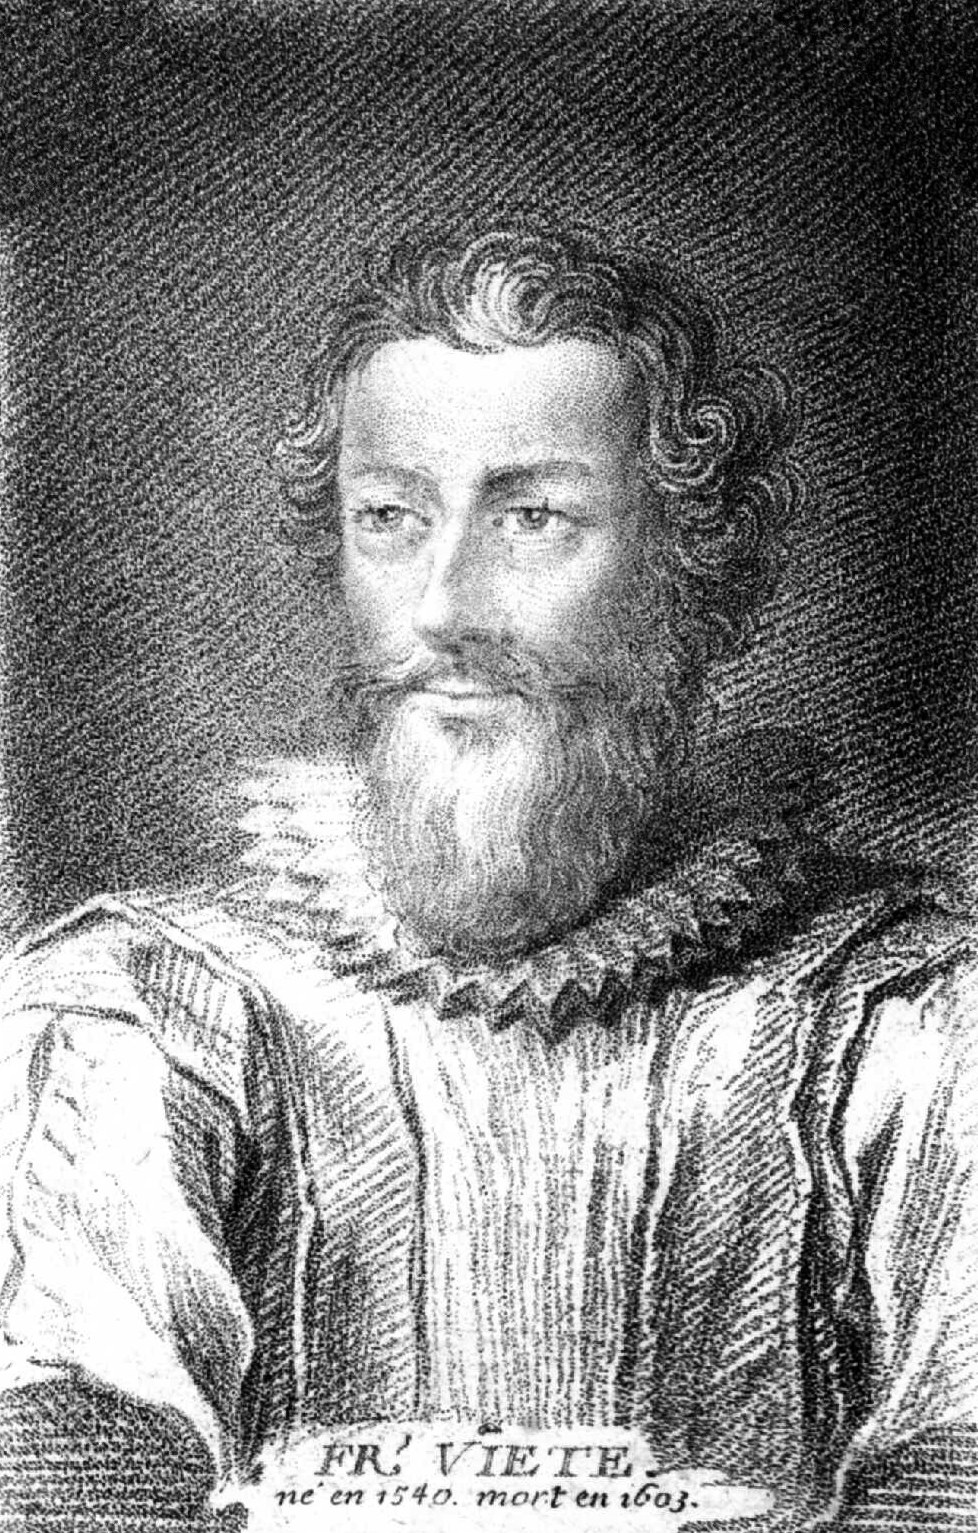
\includegraphics[width=\linewidth]{src/viete}
	\end{charbox}
	\item[Simbol Khusus Soal Latihan] Dalam soal-soal latihan, terdapat beberapa simbol khusus pada beberapa soal. Tujuan dari simbol khusus ini adalah agar pembaca dapat mengetahui jenis soal dan teknik penyelesaiannya. Beberapa simbol khusus tersebut adalah sebagai berikut.
	\begin{itemize}
		\item \probtype{$ \approx $}, yang berarti soal tersebut dapat diselesaikan dengan aproksimasi numerik.
		\item \probtype{C}, yang berarti penggunaan kalkulator (biasa) disarankan unuk menjawab soal tersebut.
		\item \probtype{CALC}, yang berarti soal tersebut kemungkinan besar harus diselesaikan dengan pengetahuan yang cukup mengenai kalkulus.
		\item \probtype{PF}, yang berarti soal tersebut selain harus diselesaikan, Anda juga harus membuktikan pekerjaan Anda.
		\item \probtype{EXPL}, yang berarti soal tersebut memerlukan eksplorasi lebih jauh mengenai materi yang telah dipelajari.
		\item \probtype{*}, \probtype{**}, dan \probtype{***} yang menunjukkan tingkat kesulitan soal tersebut.
	\end{itemize}
\end{description}
    \chapter{Daftar Notasi}

Dalam buku ini terdapat beberapa notasi matematika yang digunakan. Para mahasiswa diharapkan dapat memahami notasi-notasi tersebut agar dapat lebih memahami buku ini. Beberapa notasi tersebut adalah sebagai berikut.

\begin{enumerate}
	\item $ \mathbb{N} $ menyatakan himpunan bilangan asli, yaitu $ \lrbr{1, 2, 3, \dots} $\footnote{Terkadang ada beberapa penulis yang memasukkan 0 sebagai anggota bilangan asli.}.
	\item $ \mathbb{Z} $ menyatakan himpunan bilangan bulat, yaitu $ \lrbr{\dots, -2, -1, 0, 1, 2, \dots} $.
	\item $ \mathbb{N}_{0} $ menyatakan himpunan bilangan asli serta angka 0.
	\item $ \mathbb{Z}^{+} $ menyatakan himpunan bilangan bulat positif.
	\item $ \mathbb{Z}^{-} $ menyatakan himpunan bilangan bulat negatif.
	\item $ \mathbb{Q} $ menyatakan himpunan bilangan rasional, yaitu bilangan yang dapat dinyatakan dalam bentuk $ \frac{a}{b} $ dengan $ a $ dan $ b $ bilangan bulat serta $ b \ne 0 $.
	\item $ \mathbb{R} $ menyatakan himpunan bilangan real, yaitu bilangan yang dapat dituliskan dalam bentuk desimal.
\end{enumerate}

    \cleartorecto%
    
    {
    	\hypersetup{linkcolor=black}%
    	\tableofcontents*    % Or \tableofcontents*
    }

    \mainmatter         % Folios in Arabic numerals, numbered chapters.

    \chapter{Pendahuluan}
\label{sec:intro}

Dalam modul aljabar ini, terdapat tiga materi yang akan dibahas secara mendalam. Ketiga materi tersebut adalah persamaan dan fungsi kuadrat, pertidaksamaan satu variabel, serta eksponen dan logaritma. Sebelum mempelajari lebih mendalam mengenai ketiga materi tersebut, mahasiswa diharapkan mengetahui terlebih dahulu operasi-operasi aljabar serta simbol-simbol matematika, terutama himpunan. Pengetahuan yang cukup mengenai operasi-operasi aljabar akan mempermudah mahasiswa dalam memahami buku ini, bahkan hingga semester-semester berikutnya. Sedangkan pengetahuan yang cukup mengenai himpunan akan membantu mahasiswa dalam memahami materi pertidaksamaan.

\section{Operasi-operasi Aljabar}

Aljabar selalu membahas mengenai simbol-simbol matematika dan aturan-aturannya dalam memanipulasi simbol-simbol ini. Dalam aljabar, ada yang disebut sebagai variabel dan konstanta. Variabel adalah sesuatu yang dapat berubah-ubah. Variabel biasanya disimbolkan dengan huruf-huruf seperti $ x $, $ y $, $ \alpha $, $ \xi $, dan lain sebagainya. Sedangkan konstanta adalah suatu nilai yang tetap seperti 1, 2, $ \pi $, 0, dan bilangan-bilangan lainnya.

\begin{explbox}
	Misalnya kita diberikan $ x = 5 $, apakah $ x $ suatu konstanta atau variabel?
\end{explbox}

\par Terdapat empat operasi dasar aljabar, yaitu penjumlahan, pengurangan, perkalian, dan pembagian. Meskipun dalam buku teks matematika lebih lanjut penjumlahan dan pengurangan dianggap sama, serta perkalian dan pembagian juga dianggap sama, tetapi dalam buku ini kita anggap mereka semuanya berbeda agar lebih simpel dan mudah dipahami.

\par Terdapat istilah matematika juga yang perlu diketahui, yaitu ekspresi aljabar. Ekspresi aljabar adalah kombinasi simbol-simbol yang biasanya terdiri dari gabungan antara variabel, konstanta, dan operasi-operasi aljabar seperti penjumlahan, pengurangan, perkalian, pembagian, dan lain sebagainya. Contoh dari ekspresi aljabar ini adalah $ 2 \cdot x $, yang terdiri dari konstanta, variabel, dan operasi perkalian yang dinotasikan dengan tanda titik ditengah ($ \cdot $). Dari sini, kita bisa yakinkan diri kita bahwa konstanta dan variabel tidak dapat disatukan tanpa suatu operasi aljabar. Oleh karena itu, pembahasan mengenai operasi-operasi aljabar ini sangat diperlukan.

\par Contoh lain dari ekspresi aljabar adalah $ 2x + 3y $. Operasi-operasi ini bisa dipecah menjadi dua bagian, yaitu $ 2x $ dan $ + 3y $. Bagian-bagian inilah yang biasa disebut sebagai suku-suku dari suatu ekspresi aljabar\footnote{Meskipun sebenarnya $ 2x + 3y $ juga dapat disebut satu suku jika kita memisalkan $ u = 2x + 3y $.}. Tetapi, biasanya tanda tambah ($ + $) tidak diikutsertakan dalam pemecahan tersebut sehingga biasanya dituliskan sebagai $ 3y $ saja. Perhatikan bahwa suku-suku adalah pemecahan suatu ekspresi aljabar terhadap operasi penjumlahan dan pengurangan. Oleh karena itu, $ 2x $ disini tidak dipecah lagi menjadi dua ekspresi berbeda (yaitu 2 dan $ x $). Angka 2 pada ekspresi $ 2x $ dan angka 3 pada ekspresi $ 3x $ disebut sebagai koefisien. Bisa dibilang bahwa koefisien ini adalah angka yang berada di "depan" variabel, meskipun sebenarnya adalah angka yang dikalikan dengan suatu variabel karena angka 7 pada ekspresi $ x \cdot 7 $ juga disebut sebagai koefisien karena sesungguhnya $ x \cdot 7 = 7x $.

\par Dalam materi ini, mahasiswa diasumsikan telah mengerti mengenai operasi-operasi aljabar dan tata cara pengoperasiannya. Tetapi perlu digaris bawahi kesalahan-kesalahan yang sering dilakukan oleh mahasiswa dalam mengoperasikan suatu ekspresi aljabar, yaitu sebagai berikut:
\begin{enumerate}
	\item $ \sqrt{x + y} \stackrel{?}{=} \sqrt{x} + \sqrt{y} $;
	\item $ \dfrac{1}{x + y} \stackrel{?}{=} \dfrac{1}{x} + \dfrac{1}{y} $;
	\item $ \left(x + y\right)^{2} \stackrel{?}{=} x^{2} + y^{2} $
	\item $ \dfrac{x}{a} - \dfrac{2x + y}{a} \stackrel{?}{=} \dfrac{-x + y}{a} $; dan
	\item $ \dfrac{2x}{x} \stackrel{?}{=} 2 $.
\end{enumerate}

\begin{explbox}
	Dapatkah Anda memberikan suatu penjelasan mengenai kesalahan-kesalahan ini? Lalu bagaimana penulisan yang benar?
\end{explbox}

\section{Himpunan}

Sampai saat ini, belum ada definisi yang tepat untuk himpunan sehingga secara matematis, himpunan tidak didefinisikan. Meskipun demikian, terdapat beberapa definisi yang tidak formal mengenai himpunan. Bisa dikatakan bahwa himpunan adalah koleksi dari objek-objek yang memiliki karakteristik tertentu yang jelas seperti himpunan mahasiswa Pendidikan Matematika yang mengambil mata kuliah Aljabar. Oleh karena itu, kumpulan dari objek-objek yang belum jelas (masih merupakan pendapat pribadi atau persepsi seseorang) bukan termasuk dalam suatu himpunan, sebagai contoh kumpulan orang-orang yang tinggi bukan merupakan himpunan karena setiap orang memiliki persepsi tersendiri mengenai ketinggian seseorang.

\par Himpunan biasanya dilambangkan oleh huruf besar (misalnya $ A $, $ B $, $ \Gamma $), huruf bergaris ganda (misalnya $ \mathbb{R} $ yang melambangkan himpunan bilangan real dan $ \mathbb{Z} $ yang melambangkan himpunan bilangan bulat), atau huruf berkaligrafi (misalnya $ \mathcal{P} $ dan $ \mathcal{R} $). Sementara itu, anggota dari suatu himpunan biasanya dilambangkan oleh huruf kecil seperti $ a $, $ x $, dan $ \delta $. Keanggotaaan suatu objek dilambangkan dengan tanda "$ \in $" yang pertama kali diperkenalkan oleh Peano (1889) dan lambang untuk ketidakanggotaan adalah "$ \notin $". Misalnya, jika kita diberikan suatu himpunan $ A = \lrbr{c, d} $, maka $ c \in A $ dan $ a \notin A $.

\par Kita tidak membicarakan secara mendetail mengenai himpunan karena akan dibahas mendalam pada mata kuliah Pengantar Dasar Matematika. Pada bagian ini kita hanya membahas mengenai dasar-dasar mengenai himpunan dan notasi-notasinya serta cara mengoperasikan notasi-notasi tersebut.

\par Himpunan dapat direpresentasikan dengan dua cara, yaitu dengan cara enumerasi/pendaftaran dan dengan menggunakan notasi pembentuk himpunan. Pada cara enumerasi, semua elemen (anggota himpunan) dituliskan dan diletakkan diantara kurung kurawal. Sebagai contoh, himpunan bilangan prima yang lebih kecil dari 10 bisa dituliskan sebagai $ \lrbr{2, 3, 5, 7} $. Sementara itu, dengan menggunakan notasi pembentuk himpunan, diantara kurung kurawal diletakkan variabel, kemudian dibatasi dengan tanda "$ | $" dan dituliskan sifat yang mengatur variabel tersebut. Sebagai contoh, himpunan bilangan prima yang lebih kecil dari 10 dapat dituliskan sebagai $ \set{x}{x \mbox{ prima}, x < 10} $.

\par Kadangkala, terdapat suatu himpunan yang tidak memiliki anggota, seperti himpunan semua mahasiswa Hukum yang mengambil mata kuliah Aljabar. Berkaitan dengan hal ini, kita tuliskan himpunan yang tidak memiliki anggota tersebut dengan simbol $ \emptyset $ atau $ \lrbr{} $.

\begin{explbox}
	Diberikan himpunan $ A = \lrbr{\emptyset} $. Apakah $ A $ himpunan kosong?
\end{explbox}

\par Terdapat tiga operasi yang bisa dilakukan pada himpunan, yaitu gabungan, irisan, dan selisih\footnote{Sebenarnya masih banyak lagi operasi-operasi pada himpunan seperti \textit{symmetric difference}. Untuk persiapan menghadapi mata kuliah Aljabar ini, operasi tersebut tidak terlalu sering digunakan sehingga dilewatkan pembahasannya.}. Ketiga operasi tersebut didefinisikan sebagai berikut.

\paragraph{Definisi 1.2.1 \label{def121}} Misalkan $ A $ dan $ B $ himpunan. Maka,
\begin{enumerate}
	\item Gabungan dari $ A $ dan $ B $ yang dilambangkan dengan $ A \cup B $ didefinisikan sebagai
	\[ A \cup B \coloneqq \set{x}{x \in A \, \vee \, x \in B}. \]
	Oleh karena itu, $ x \in A \cup B $ jika dan hanya jika $ x \in A $ atau $ x \in B $. Ilustrasinya adalah sebagai berikut.
	\begin{figure}[H]
		\centering
		\begin{venndiagram2sets}
			\fillA \fillB
		\end{venndiagram2sets}
		\caption{Ilustrasi gabungan dua himpunan.}
	\end{figure}
	\item Irisan dari $ A $ dan $ B $ yang dilambangkan dengan $ A \cap B $ didefinisikan sebagai
	\[ A \cap B \coloneqq \set{x}{x \in A \, \wedge \, x \in B}. \]
	Oleh karena itu, $ x \in A \cap B $ jika dan hanya jika $ x \in A $ dan $ x \in B $. Ilustrasinya adalah sebagai berikut.
	\begin{figure}[H]
		\centering
		\begin{venndiagram2sets}
			\fillACapB
		\end{venndiagram2sets}
		\caption{Ilustrasi irisan dua himpunan.}
	\end{figure}
	\item Selisih dari $ A $ dan $ B $ yang dilambangkan dengan $ A \backslash B $ (atau kadang $ A - B $) didefinisikan sebagai
	\[ A \backslash B \coloneqq \set{x}{x \in A \, \wedge \, x \notin B}. \]
	Oleh karena itu, $ x \in A \backslash B $ jika dan hanya jika $ x \in A $ dan $ x \notin B $. Ilustrasinya adalah sebagai berikut.
	\begin{figure}[H]
		\centering
		\begin{venndiagram2sets}
			\fillANotB
		\end{venndiagram2sets}
		\caption{Ilustrasi selisih dua himpunan.}
	\end{figure}
\end{enumerate}

\par Sebagai contoh, untuk mengiris himpunan $ A = \set{x}{1 < x \leq 5} $ dan $ B \ \set{x}{x > 3} $ bisa dilakukan dengan mencari suatu himpunan $ C $ sedemikian sehingga setiap anggota di $ C $ merupakan anggota dari himpunan $ A $ dan juga merupakan anggota himpunan $ B $. Himpunan $ C $ yang memenuhi ini pastilah $ C = \set{x}{3 < x \leq 5} $. Jadi $ C = A \cap B $. Sedangkan, jika kita ingin menggabungkan $ A $ dan $ B $, maka kita perlu mencari himpunan $ D $ sedemikian sehingga setiap anggota himpunan $ D $ juga berada di $ A $ atau $ B $. Tentunya himpunan $ D $ yang memenuhi adalah $ D = \set{x}{x > 1} $.

\par Terkadang akan sangat sulit untuk mencari himpunan yang memenuhi $ A \cup B $ atau $ A \cap B $ pada contoh di atas. Oleh karena itu, kita bisa menggunakan garis bilangan real untuk mempermudah pencarian gabungan dan irisan dari dua atau lebih himpunan. Jika $ A $ dan $ B $ digambarkan pada garis bilangan real, maka tampaknya adalah sebagai berikut.
\begin{figure}[H]
	\centering
	\begin{tikzpicture}
		\begin{axis}[
			axis x line=middle,
			axis y line=none,
			axis line style=<->,
			xmin=0,
			ymin=0,
			height=2.5cm,
			width=8cm
			]
		{
			\addplot[domain=1:5, thick, blue] {1};
			\addplot[color=blue, holdot] coordinates{(1, 1)};
			\addplot[color=blue, soldot] coordinates{(5, 1)};
			
			\addplot[domain=3:7, thick, red, ->] {2};
			\addplot[color=red, holdot] coordinates{(3, 2)};
		}
		\end{axis}
	\end{tikzpicture}
	\caption{Ilustrasi $ A $ (biru) dan $ B $ (merah) jika digambarkan pada garis bilangan real.}
\end{figure}
Pada gambar di atas, $ A \cup B $ adalah segala garis bilangan yang dilewati oleh garis biru (himpunan $ A $) atau garis merah (himpunan $ B $) sehingga $ A \cup B = \set{x}{x > 1} $. Sementara itu, $ A \cap B $ adalah segala garis bilangan yang dilewati oleh garis biru (himpunan $ A $) dan garis merah (himpunan $ B $) sekaligus sehingga $ A \cap B = \set{x}{3 < x \leq 5} $.

\par Perhatikan sekali lagi pada gambar garis bilangan di atas. Jika titik ujungnya masih termasuk ke dalam suatu himpunan, maka titik ujung garis tersebut harus diberi tanda bulat penuh. Tetapi jika titik ujungnya tidak termasuk ke dalam suatu himpunan, maka titik ujung garis tersebut harus diberi tanda bulat takpenuh. Seperti pada himpunan $ A $ (garis biru), karena $ 5 \in A $ dan 5 adalah titik ujung (kanan) himpunan $ A $, maka garis yang mengilustrasikan himpunan $ A $ pada garis bilangan real diberi tanda bulatan penuh. Begitu juga sebaliknya, karena $ 1 \notin A $ dan 1 adalah titik ujung (kiri) himpunan $ A $, maka garis yang mengilustrasikan himpunan $ A $ pada garis bilangan real diberi tanda bulatan takpenuh.

\begin{explbox}
	Suatu himpunan juga dapat dinyatakan dalam notasi interval. Coba cari tahu mengenai notasi interval tersebut!
\end{explbox}

\par Dalam bekerja dengan menggunakan himpunan, kita harus mengetahui sedang membicarakan apa. Pada penjelasan-penjelasan mengenai himpunan sebelumnya, seperti pada himpunan $ A $ dan $ B $ pada contoh di atas, kita tidak diberikan informasi mengenai variabel $ x $. Kita tidak mengetahui apakah $ x $ termasuk bilangan real, bilangan rasional, atau bilangan bulat. Oleh karena itu, selanjutnya kita harus menspesifikasikan variabel yang bekerja pada suatu himpunan. Jika $ x $ merupakan bilangan bulat, maka penulisan himpunan yang benar adalah $ A = \set{x \in \mathbb{Z}}{1 < x \leq 5} $. Sementara itu, jika $ x $ merupakan bilangan real, maka penulisan himpunan yang benar adalah $ A = \set{x \in \mathbb{R}}{1 < x \leq 5} $. Begitu pula jika $ x $ rasional, $ x $ bilangan asli, atau yang lainnya.

\subsection{Latihan Soal 1.2}
\begin{enumerate}[leftmargin=*]
	\item Buatlah tabel mengenai seluruh kemungkinan interval dan himpunan yang berkaitan beserta ilustrasi pada garis bilangan realnya.
	\item Jika $ A = \set{x \in \mathbb{R}}{x \leq 1} $ dan $ B = \set{x \in \mathbb{Z}}{-2 < x < 3} $, maka tentukanlah $ A \cup B $, $ A \cap B $, dan $ A \backslash B $.
	\item Diberikan himpunan $ \mathcal{P} $ dan $ \mathcal{Q} $. Buatlah suatu ilustrasi mengenai $ \mathcal{P} \backslash \mathcal{Q} $ yang digambarkan pada garis bilangan real untuk tiga himpunan $ \mathcal{P} $ dan $ \mathcal{Q} $ yang berbeda.
	\item Jika $ A $ dan $ B $ adalah sebarang himpunan takkosong, mungkinkah $ A \cup B $ merupakan himpunan kosong? Berikan suatu contoh mengenai hal ini.
	\item Tentukan interval paling sederhana yang ekuivalen dengan
	\[ \left(\left(-15, 20\right) \cup \lrbr{20}\right) \backslash \left(\left[4, 5\right] \cap \lkrb{2, +\infty}\right). \]
	Ilustrasikan pekerjaan Anda dengan membuat interval-interval tersebut pada garis bilangan real.
\end{enumerate}

\section{Identitas Aljabar}

Akan sangat membantu jika Anda mengetahui identitas-identitas aljabar dalam mata kuliah ini. Identitas-identitas aljabar ini dapat membantu meringankan beban Anda dalam menghitung suatu ekspresi matematika yang rumit. Berikut merupakan identitas-identitas yang sering digunakan untuk membantu menyelesaikan permasalahan matematika.
\begin{enumerate}
	\item $ x^{2} + y^{2} = \left(x + y\right)^{2} - 2xy = \left(x - y\right)^{2} + 2xy = \dfrac{1}{2}\left(\left(x + y\right)^{2} + \left(x - y\right)^{2}\right) $
	\item $ x^{2} - y^{2} = \left(x + y\right)\left(x - y\right) $
	\item $ x^{3} + y^{3} = \left(x + y\right)\left(x^{2} - xy + y^{2}\right) $
	\item $ x^{3} - y^{3} = \left(x - y\right)\left(x^{2} + xy + y^{2}\right) $
	\item Untuk setiap bilangan bulat positif ganjil $ n $,
	\[ x^{n} + y^{n} = \left(x + y\right)\left(x^{n - 1} - x^{n - 2}y + \cdots - xy^{n - 2} + y^{n - 1}\right). \]
	\item Untuk setiap bilangan bulat positif genap $ n $,
	\[ x^{2} + y^{n} = \left(x - y\right)\left(x^{n - 1} + x^{n - 2}y + \cdots + x^{n - 2}y + y^{n - 1}\right). \]
	\item Untuk setiap bilangan bulat positif $ n $,
	\[ x^{n} - y^{n} = \left(x - y\right)\left(x^{n - 1} + x^{n - 2}y + \cdots + xy^{n - 2} + y^{n - 1}\right). \]
	\item $ x^{3} + y^{3} + z^{3} - 3xyz = \left(x + y + z\right)\left(x^{2} + y^{2} + z^{2} - xy - yz - xz\right) = \dfrac{1}{2}\left(x + y + z\right)\left(\left(x - y\right)^{2} + \left(y - z\right)^{2} + \left(z - x\right)^{2}\right) $
	\item Untuk setiap bilangan bulat positif $ n \geq 2 $,
	\[ \left(x_{1} + x_{2} + \cdots + x_{n}\right)^{2} = x_{1}^{2} + x_{2}^{2} + \cdots + x_{n}^{2} + 2\left(x_{1}x_{2} + x_{2}x_{3} + \cdots + x_{n - 1}x_{n} + x_{n}x_{1}\right). \]
	\item $ \left(ax + by\right)^{2} \pm \left(ay \mp bx\right)^{2} = \left(a^{2} \pm b^{2}\right)\left(x^{2} \pm y^{2}\right) $
	\item $ x^{2}y + y^{2}z + z^{2}x + x^{2}z + y^{2}x + z^{2}y + 2xyz = \left(x + y\right)\left(y + z\right)\left(z + x\right) $
	\item $ a^{4} + 4b^{4} = \left(a^{2} + 2b^{2} - 2ab\right)\left(a^{2} + 2b^{2} + 2ab\right) $
\end{enumerate}

\subsection{Latihan Soal 1.3}
\begin{enumerate}[leftmargin=*]
	\item Uji kebenaran identitas-identitas pada subbab ini.
	\item Cari tahu mengenai Simon's Favorite Factoring Trick (SFFT). Apa kaitannya dengan identitas-identitas di atas?
	\item Faktorkanlah ekspresi aljabar $ \left(x - y\right)^{3} + \left(y - z\right)^{3} + \left(z - x\right)^{3} $.
\end{enumerate}

    \chapter{Persamaan Kuadrat dan Fungsi Kuadrat}
\label{sec:second}

%% Subbab 1 %%

\section{Persamaan Kuadrat}

Persamaan adalah kalimat terbuka yang dihubungkan oleh tanda kesamaan ($ = $). Artinya, suatu persamaan belum diketahui nilai kebenarannya. Sebagai contoh, $ 2x + 3 = 5 $ merupakan persamaan. Kita tidak mengetahui apakah persamaan tersebut benar untuk beberapa nilai $ x $. Jika $ x = 1 $, maka persamaan tersebut bernilai benar sehingga persamaan tersebut menjadi suatu kesamaan (kalimat tertutup yang bernilai benar). Tetapi, jika $ x \ne 1 $, maka persamaan tersebut akan selalu bernilai salah sehingga persamaan tersebut menjadi suatu ketaksamaan (kalimat tertutup yang bernilai salah). Dalam hal ini, $ x = 1 $ kadang disebut sebagai solusi\footnote{Terkadang juga disebut sebagai akar atau penyelesaian.} dari persamaan $ 2x + 3 = 5 $.

\par Persamaan kuadrat merupakan salah satu dari banyak jenis persamaan dalam matematika. Persamaan kuadrat memiliki bentuk umum
\begin{equation} \label{eq:201}
	ax^{2} + bx + c = 0
\end{equation}
dengan $ a, b, c \in \mathbb{R} $ dan $ a \ne 0 $.

\begin{explbox}
	Mengapa dalam persamaan kuadrat haruslah $ a \ne 0 $?
\end{explbox}

\par Dalam persamaan kuadrat $ 3x^{2} + 2x - 5 = 0 $, nilai $ a = 3 $, $ b = 2 $, dan $ c = -5 $. Sedangkan pada persamaan kuadrat $ -3x^{2} + 10 = 0 $, nilai $ a = -3 $, nilai $ b = 0 $, dan nilai $ c = 10 $. Hal ini dikarenakan kita dapat menuliskan ekspresi $ -3x^{2} + 10 $ sebagai $ -3x^{2} + 0x + 10 $. Lalu bagaimana dengan persamaan $ x^{2} = -1 $?

\par Meskipun persamaan kuadrat memiliki bentuk umum seperti yang dapat dilihat pada persamaan \ref{eq:201}, persamaan seperti $ 2x + 3 = 0 $ juga dapat dipandang sebagai persamaan kuadrat, namun dalam $ \sqrt{x} $. Jika kita misalkan $ \sqrt{x} = u $, maka $ 2x + 3 = 0 $ dapat ditulis sebagai $ 2u^{2} + 3 = 0 $ yang merupakan persamaan kuadrat dalam $ u $ atau $ \sqrt{x} $.

\subsection{Cara Mencari Solusi Persamaan Kuadrat}

	Persamaan kuadrat tentunya memiliki solusi. Ingat kembali bahwa solusi adalah suatu nilai yang menyebabkan suatu persamaan menjadi kesamaan. Oleh karena itu, jika $ x = p $ merupakan solusi dari persamaan kuadrat umum \ref{eq:201}, maka $ ap^{2} + bp + c = 0 $. Tetapi, bagaimana cara menentukan solusinya? Dalam menyelesaikan suatu persamaan kuadrat, terdapat tiga cara yang dapat digunakan. Ketiga cara tersebut adalah dengan menggunakan faktorisasi, melengkapkan kuadrat, dan dengan menggunakan rumus kuadratik (rumus abc). Berikut merupakan penjelasannya.
	
	\subsubsection{Faktorisasi}
	
		Persamaan kuadrat umum seperti pada persamaan \ref{eq:201} dapat difaktorkan menjadi
		\begin{equation} \label{eq:202}
			a\left(x - p\right)\left(x - q\right) = 0.
		\end{equation}
		Disini, $ p $ dan $ q $ bisa jadi bukan termasuk bilangan real. Tetapi dalam buku ini, kita tidak akan membahas mengenai pemfaktoran dimana $ p $ dan $ q $ bukan bilangan real sehingga kita bisa anggap $ p, q \in \mathbb{R} $. Untuk lebih jauhnya mengenai hal ini akan dibahas pada bagian selanjutnya.
		
		\par Perhatikan kembali persamaan \ref{eq:202}. Jika kita substitusi $ x = p $, maka ruas kiri akan sama dengan nol. Tetapi, jika kita substitusi $ x = q $, maka ruas kiri juga akan menjadi nol. Oleh karena itu, $ p $ dan $ q $ merupakan akar-akar dari persamaan \ref{eq:202}. Dalam hal ini, kita tuliskan akar-akar dari persamaan \ref{eq:202} adalah $ x = p $ atau $ x = q $ (mengapa bukan 'dan'?). Jika kita pandang $ p $ sebagai akar pertama dan $ q $ sebagai akar kedua dari persamaan \ref{eq:202}, maka kita dapat tuliskan akar-akar dari persamaan $ \ref{eq:202} $ adalah $ x_{1} = p $ dan $ x_{2} = q $ (mengapa bukan 'atau'?).
		
		\par Pada persamaan \ref{eq:201}, jika $ a = 1 $, maka persamaan tersebut dapat ditulis sebagai
		\begin{equation} \label{eq:203}
			x^{2} + bx + c = 0.
		\end{equation}
		Perhatikan bahwa kita dapat memfaktorkan persamaan \ref{eq:203} menjadi
		\begin{equation} \label{eq:204}
			\left(x + p\right)\left(x + q\right) = 0
		\end{equation}
		dengan $ p $ dan $ q $ bilangan-bilangan real yang jika dijabarkan akan diperoleh
		\[ x^{2} + \left(p + q\right)x + pq = 0. \]
		Jadi, agar persamaan \ref{eq:203} ekuivalen dengan persamaan \ref{eq:204}, maka haruslah kita mencari $ p $ dan $ q $ sedemikian sehingga $ p + q = b $ dan $ pq = c $.
		
		\begin{contoh}
			Selesaikan persamaan kuadrat $ x^{2} - 7x + 10 = 0 $.
		\end{contoh}
		\begin{jawab}
			Jika kita ingin memfaktorkan ruas kiri persamaan pada soal menjadi $ \left(x + p\right)\left(x + q\right) = 0 $, maka kita harus mencari $ p $ dan $ q $ sedemikian sehingga $ p + q = -7 $ dan $ pq = 10 $. Setelah mencoba-coba, ternyata $ p = -2 $ dan $ q = -5 $ memenuhi. Oleh karena itu, kita dapat menulis ulang persamaan pada soal sebagai
			\[ \left(x - 2\right)\left(x - 5\right) = 0. \]
			Jadi, solusi persamaan kuadrat pada soal adalah $ x = 2 $ atau $ x = 5 $.
		\end{jawab}
		
		\par Pada persamaan \ref{eq:201}, jika $ a \ne 1 $, maka secara umum kita dapat menyelesaikannya dengan langkah-langkah sebagai berikut.
		\begin{enumerate}
			\item Pertama-tama, persamaan \ref{eq:201} kita faktorkan menjadi
			\begin{equation} \label{eq:205}
				\frac{\left(ax + p\right)\left(ax + q\right)}{a} = 0.
			\end{equation}
			\item Selanjutnya, carilah nilai $ p $ dan $ q $ sedemikian sehingga $ p + q = b $ dan $ pq = ac $.
			\item Setelah didapatkan nilai $ p $ dan $ q $, substitusikan kembali ke persamaan \ref{eq:205} dan sederhanakan lebih lanjut.
		\end{enumerate}
		
		\begin{explbox}
			Uji kebenaran langkah-langkah pemfaktoran di atas. Mengapa langkah-langkah tersebut benar?
		\end{explbox}
		
		\begin{contoh}
			Selesaikan persamaan kuadrat $ 2x^{2} - 5x - 3 = 0 $.
		\end{contoh}
		\begin{jawab}
			Pertama-tama, persamaan pada soal kita faktorkan menjadi
			\[ \frac{\left(2x + p\right)\left(2x + q\right)}{2} = 0. \]
			Selanjutnya, kita cari nilai $ p $ dan $ q $ sedemikian sehingga $ p + q = -5 $ dan $ pq = -6 $. Setelah mencoba-coba, ternyata $ p = 1 $ dan $ q = -6 $ memenuhi. Oleh karena itu, kita dapat menulis ulang pemfaktoran terakhir sebagai
			\[ \frac{\left(2x + 1\right)\left(2x - 6\right)}{2} = 0 \iff \left(2x + 1\right)\left(x - 3\right) = 0. \]
			Agar persamaan terakhir bernilai benar, maka $ 2x + 1 = 0 \iff x = -\dfrac{1}{2} $ atau $ x - 3 = 0 \iff x = 3 $.
			\par \noindent Jadi, solusi persamaan kuadrat pada soal adalah $ x = -\dfrac{1}{2} $ atau $ x = 3 $.
		\end{jawab}
		
		\begin{warningbox}
			Jika Anda ingin mencari solusi dari persamaan $ x^{2} = 9 $, Anda tidak boleh langsung menarik akar pada kedua ruas sehingga didapatkan $ x = 3 $. Hal ini dikarenakan, $ x = -3 $ juga memenuhi persamaan tersebut. Beberapa cara untuk memunculkan solusi $ x = -3 $ adalah dengan menambahkan tanda '$ \pm $' di ruas kanan persamaan setelah ditarik akarnya seperti $ x^{2} = 9 \implies x = \pm 3 $ sehingga solusinya adalah $ x = 3 $ atau $ x = -3 $. Anda juga dapat mengurangi kedua ruas dengan tiga, lalu memfaktorkannya dengan identitas selisih kuadrat seperti
			\[ x^{2} = 9 \iff x^{2} - 9 = 0 \iff \left(x + 3\right)\left(x - 3\right) = 0 \]
			sehingga solusinya adalah $ x = 3 $ atau $ x = -3 $.
		\end{warningbox}
		
	\subsubsection{Melengkapkan Kuadrat}
	
		Terkadang, kita akan kesulitan untuk memfaktorkan suatu bentuk kuadrat. Sebagai contoh, Anda dapat mencoba memfaktorkan ekspresi $ x^{2} + x + 1 $ ini. Anda pasti akan kesulitan memfaktorkan ekspresi tersebut. Oleh karena itu, teknik melengkapkan kuadrat akan sangat membantu disini. Teknik ini sangatlah berguna untuk menyelesaikan suatu persamaan kuadrat yang sukar untuk difaktorkan.
		
		\par Melengkapkan kuadrat adalah suatu teknik untuk mengubah bentuk persamaan kuadrat umum seperti pada persamaan \ref{eq:201} menjadi suatu persamaan kuadrat berbentuk
		\begin{equation} \label{eq:206}
			a\left(x + h\right)^{2} + k = 0.
		\end{equation}
		untuk suatu bilangan real $ h $ dan $ k $. Dalam bentuk ini, persamaan kuadrat akan jauh lebih mudah untuk diselesaikan dibandingkan pada bentuk umumnya.
		
		\par Jika $ a = 1 $, tentunya proses melengkapkan kuadrat akan mudah. Misalkan $ a = 1 $, maka persamaan \ref{eq:201} dapat dituliskan sebagai
		\[ x^{2} + bx + c = 0 \]
		seperti yang terdapat pada persamaan \ref{eq:203}.
		\par \noindent Perhatikan bahwa $ \left(x + \dfrac{1}{2}b\right)^{2} = x^{2} + bx + \left(\dfrac{b}{2}\right)^{2} $. Oleh karena itu, kita harus munculkan bentuk $ \left(\dfrac{b}{2}\right)^{2} $ pada persamaan \ref{eq:203} dengan menjumlahkan kedua ruas dengan bentuk tersebut. Oleh karena itu, persamaan \ref{eq:203} dapat kita tulis ulang sebagai
		\[ x^{2} + bx + \left(\frac{b}{2}\right)^{2} + c = \left(\frac{b}{2}\right)^{2} \iff \left(x + \frac{1}{2}b\right)^{2} + c - \left(\frac{b}{2}\right)^{2} = 0. \]
		Dengan membandingan koefisien-koefisien ruas kiri persamaan terakhir dengan ruas kiri persamaan \ref{eq:206}, kita dapatkan $ h = \dfrac{b}{2} $ dan $ k = c - \left(\dfrac{b}{2}\right)^{2} $.
		
		\begin{contoh}
			Dengan melengkapkan kuadrat, tentukan penyelesaian dari persamaan $ x^{2} + 4x - 9 = 0 $.
		\end{contoh}
		\begin{jawab}
			Karena $ b = 4 $ dan $ c = -9 $, maka $ h = \dfrac{1}{2}\left(4\right) = 2 $. Oleh karena itu, kita bisa menjumlahkan kedua ruas dengan $ 2^{2} = 4 $ sehingga
			\[ x^{2} + 4x + 4 - 9 = 4 \iff \left(x + 2\right)^{2} = 13. \]
			Menarik akar kedua ruas akan didapatkan
			\[ x + 2 = \pm 13 \iff x = -2 \pm 13. \]
			Jadi solusi persamaan kuadrat pada soal adalah $ x = -2 - \sqrt{13} $ atau $ x = -2 + \sqrt{13} $.
		\end{jawab}
		
		\par Jika $ a \ne 1 $, kita dapat mencoba untuk membagi kedua ruas persamaan kuadrat dengan $ a $. Sebagai contoh, kita akan mengerjakan soal berikut.
		
		\begin{contoh}
			Dengan melengkapkan kuadrat, tentukan penyelesaian dari persamaan $ 2x^{2} + 3x + 1 = 0 $.
		\end{contoh}
		\begin{jawab}
			Dengan membagi kedua ruas dengan 2, kita akan mendapatkan
			\[ x^{2} + \frac{3}{2}x + \frac{1}{2} = 0. \]
			Sampai disini, proses untuk melengkapkan kuadrat sama seperti contoh sebelumnya dan diserahkan kepada pembaca sebagai latihan.
		\end{jawab}
		
		\par Terkadang, membagi kedua ruas dengan $ a $ akan menimbulkan masalah baru seperti rumitnya proses melengkapkan kuadrat karena harus berurusan dengan pecahan yang bentuknya ekstrim. Oleh karena itu, alih-alih membagi kedua ruas dengan $ a $, kita juga bisa mencoba untuk mengalikan kedua ruas dengan $ a $ sehingga akan didapatkan persamaan kuadrat baru dalam $ ax $. Sebagai contoh, kita akan mengerjakan soal berikut.
		
		\begin{contoh}
			Dengan melengkapkan kuadrat, tentukan penyelesaian dari persamaan $ 3x^{2} + x - 5 = 0 $.
		\end{contoh}
		\begin{jawab}
			Dengan mengalikan kedua ruas dengan 3, kita akan mendapatkan
			\[ 3^{2}x^{2} + 3x - 5 = 0 \iff \left(3x\right)^{2} + 3x - 5 = 0. \]
			Misalkan $ 3x = u $, maka kita bisa tulis ulang persamaan terakhir sebagai
			\[ u^{2} + u - 5 = 0. \]
			Sampai disini, proses untuk melengkapkan kuadrat sama seperti contoh sebelumnya dan diserahkan kepada pembaca sebagai latihan. Jangan lupa untuk substitusi balik $ u = 3x $.
		\end{jawab}
	
	\subsubsection{Rumus Kuadratik}
		
		Di Indonesia, rumus kuadratik sering disebut sebagai rumus abc. Rumus kuadratik sebenarnya didapatkan dengan menggunakan teknik melengkapkan kuadrat pada persamaan \ref{eq:201}. Rumus kuadratik dapat dituliskan sebagai berikut.
		
		\begin{teorema}[Rumus Kuadratik] \label{thm:21}
			Misalkan solusi-solusi dari persamaan \ref{eq:201} adalah $ x_{1, 2} $ (yang berarti $ x_{1} $ dan $ x_{2} $), maka
			\begin{equation} \label{eq:207}
				x_{1, 2} = \frac{-b \pm \sqrt{b^{2} - 4ac}}{2a}.
			\end{equation}
		\end{teorema}
		\begin{bukti}
			Membagi kedua ruas persamaan \ref{eq:201} dengan $ a $ dan dilanjutkan dengan melengkapkan kuadrat akan didapatkan
			\begin{alignat*}{2}
				&\qquad& x^{2} + \frac{b}{a}x + \frac{c}{a} &= 0 \\
				\iff&& x^{2} + \frac{b}{a}x + \left(\frac{b}{2a}\right)^{2} + \frac{c}{a} &= \left(\frac{b}{2a}\right)^{2} \\
				\iff&& \left(x + \frac{b}{2a}\right)^{2} &= \frac{b^{2}}{4a^{2}} - \frac{c}{a} \\
				\iff&& \left(x + \frac{b}{2a}\right)^{2} &= \frac{b^{2}a - 4a^{2}c}{4a^{3}} \\
				\iff&& \left(x + \frac{b}{2a}\right)^{2} &= \frac{b^{2} - 4ac}{4a^{2}} \\
				\iff&& x_{1, 2} + \frac{b}{2a} &= \pm \frac{\sqrt{b^{2} - 4ac}}{2a} \\
				\iff&& x_{1, 2} &= \frac{-b \pm \sqrt{b^{2} - 4ac}}{2a}
			\end{alignat*}
			dan kita selesai.
		\end{bukti}
	
		\begin{explbox}
			Alih-alih membagi kedua ruas dengan $ a $, coba Anda buktikan teorema \ref{thm:21} dengan mengalikan kedua ruas persamaan \ref{eq:201} dengan $ a $, lalu dilanjutkan dengan melengkapkan kuadrat.
		\end{explbox}
		
		\par Rumus kuadratik ini merupakan alat yang sangat canggih untuk menyelesaikan suatu persamaan kuadrat. Mungkin kita akan kesulitan jika menyelesaikan persamaan kuadrat dengan menggunakan pemfaktoran atau melengkapkan kuadrat, tetapi rumus kuadratik ini akan dapat membantu kita dengan cepat. Rumus kuadratik inilah yang akan membantu kita untuk memahami persamaan kuadrat lebih lanjut lagi.
		
		\begin{contoh}
			Dengan menggunakan rumus kuadratik, tentukan akar-akar dari persamaan $ 2x^{2} - x - 11 = 0 $.
		\end{contoh}
		\begin{jawab}
			Pertama, kita tentukan terlebih dahulu nilai $ a $, $ b $, dan $ c $. Dengan membandingkan koefisien-koefisien persamaan pada soal dengan persamaan \ref{eq:201}, kita dapatkan $ a = 2 $, $ b = -1 $, dan $ c = -11 $. Oleh karena itu, dengan rumus kuadratik, kita akan mendapatkan
			\[ x_{1, 2} = \frac{-\left(-1\right) \pm \sqrt{\left(-1\right)^{2} - 4\left(2\right)\left(-11\right)}}{2\left(2\right)} = \frac{1 \pm \sqrt{1 + 88}}{4} = \frac{1 \pm \sqrt{89}}{4} \]
			sehingga akar-akar persamaan pada soal adalah
			\[ x_{1} = \frac{1 + \sqrt{89}}{4} \quad \mbox{dan} \quad x_{2} = \frac{1 - \sqrt{89}}{4}. \]
		\end{jawab}
		
		\par Dari rumus kuadratik ini, kita dapat memfaktoran bentuk kuadrat $ ax^{2} + bx + c $ sebagai
		\[ a\left(x - \frac{-b + \sqrt{b^{2} - 4ac}}{2a}\right)\left(x - \frac{-b - \sqrt{b^{2} - 4ac}}{2a}\right) \]
		dan pada kasus khusus jika $ b^{2} = 4ac $, kita dapat memfaktorkan bentuk kuadrat $ ax^{2} + bx + c $ sebagai
		\[ a\left(x + \frac{b}{2a}\right)^{2}. \]
		
		\begin{explbox}
			Coba cari tahu mengenai persamaan kuadratik tereduksi. Bagaimanakah rumus kuadratik digunakan dalam persamaan tersebut?
		\end{explbox}
	
\subsection{Diskriminan}

	Dalam persamaan kuadrat, diskriminan adalah ekspresi yang berada di bawah tanda akar pada rumus kuadratik seperti pada teorema \ref{thm:21}. Diskriminan sering disimbolkan sebagai huruf kapital $ D $ atau huruf kapital Yunani $ \Delta $ (delta kapital)\footnote{Di Indonesia sendiri, notasi yang sering digunakan untuk diskriminan adalah $ D $ sehingga selanjutnya kita akan menotasikan diskriminan sebagai $ D $, kecuali ada keterangan lain.} dimana
	\begin{equation} \label{eq:208}
		D = \Delta = b^{2} - 4ac.
	\end{equation}
	dengan $ a, b, c $ berturut-turut merupakan koefisien-koefisien persamaan kuadrat umum \ref{eq:201}. Oleh karena itu, formula \ref{eq:207} dapat dituliskan sebagai
	\begin{equation} \label{eq:209}
		x_{1, 2} = \frac{-b \pm \sqrt{D}}{2a}.
	\end{equation}
	
\subsection{Jenis-jenis Akar Persamaan Kuadrat}

	Terdapat dua kemungkinan akar-akar yang mungkin untuk persamaan kuadrat. Dua kemungkinan ini bergantung pada nilai diskriminan pada persamaan kuadrat tersebut. Jika $ D < 0 $, maka akar-akar persamaan kuadrat tersebut bukan merupakan bilangan real (bilangan kompleks, yang kadang dinotasikan sebagai $ \mathbb{C} $), tetapi jika $ D \geq 0 $, maka akar-akar persamaan kuadrat tersebut merupakan bilangan real.
	
	\par Jika $ D < 0 $, maka nilai di dalam akar pada persamaan \ref{eq:209} akan bernilai negatif. Padahal nilai di dalam akar harus nonnegatif agar nilainya terdefinisi pada garis bilangan real. Oleh karena itu, akar-akar yang dihasilkan oleh persamaan kuadrat yang diskriminannya negatif akan bernilai tidak real. Lain halnya jika $ D \geq 0 $. Nilai di dalam akar pada persamaan \ref{eq:209} akan bernilai nonnegatif yang sudah pasti nilainya akan terdefinisi pada garis bilangan real.
	
	\par Biasanya jika suatu persamaan kuadrat memiliki diskriminan negatif, kita tidak akan mencari akar-akarnya secara eksplisit. Hal ini dikarenakan ruang lingkup pembicaraan kita yang terbatas hanya untuk bilangan real. Tetapi jika Anda memiliki keingintahuan yang tinggi, Anda dapat mencoba untuk menyelesaikannya dengan menggunakan rumus kuadratik. Tetapi untuk menyelesaikannya, Anda perlu mengetahui terlebih dahulu mengenai bilangan imajiner. Sebagai contoh, misalkan kita diberikan suatu persamaan kuadrat $ x^{2} + x + 1 = 0 $. Diskriminan persamaan kuadrat tersebut adalah $ D = 1^{2} - 4\left(1\right)\left(1\right) = -3 $. Oleh karena itu, dengan menggunakan rumus kuadratik kita akan mendapatkan
	\[ x_{1, 2} = \frac{-1 \pm \sqrt{-3}}{2}. \]
	Untuk menghadapi akar dengan ekspresi di dalam akar yang bernilai negatif, kita perlu untuk menguraikannya terlebih dahulu. Dalam hal ini, kita uraikan $ -3 $ sebagai $ -1 \cdot 3 $. Oleh karena itu, $ \sqrt{-3} = \sqrt{-1 \cdot 3} = \sqrt{3} \cdot \sqrt{-1} $. Dalam matematika, biasanya kita notasikan $ \sqrt{-1} $ sebagai $ i $ sehingga $ \sqrt{3} \cdot \sqrt{-1} = \sqrt{3}i $. Bilangan $ i $ inilah yang disebut sebagai bilangan imajiner. Oleh karena itu,
	\[ x_{1, 2} = \frac{-1 \pm \sqrt{3}i}{2} \]
	sehingga akar-akar persamaan kuadrat $ x^{2} + x + 1 = 0 $ adalah
	\[ x_{1} = \frac{-1 + \sqrt{3}i}{2} \quad \mbox{dan} \quad x_{2} = \frac{-1 - \sqrt{3}i}{2}. \]
	
	\par Persamaan kuadrat yang memiliki diskriminan nonnegatif dibagi lagi menjadi dua jenis, yaitu persamaan kuadrat dengan diskriminan nol dan persamaan kuadrat dengan diskriminan positif. Jika suatu persamaan kuadrat memiliki nilai $ D = 0 $, maka persamaan \ref{eq:209} dapat dituliskan sebagai
	\[ x_{1, 2} = -\frac{b \pm 0}{2a} = -\frac{b}{2a}. \]
	Akibatnya, $ x_{1} = x_{2} = -\dfrac{b}{2a} $ sehingga persamaan kuadrat tersebut memiliki tepat satu akar real. Terkadang juga disebut akarnya berulang atau akarnya ganda. Hal ini akan dibahas pada bagian tersendiri untuk lebih memahaminya lebih lanjut. Selain itu, jika suatu persamaan kuadrat memiliki nilai $ D > 0 $, maka persamaan kuadrat tersebut memiliki dua akar yang berbeda, yaitu
	\[ x_{1} = -\frac{-b + \sqrt{D}}{2a} \quad \mbox{dan} \quad x_{2} = \frac{-b - \sqrt{D}}{2a} \]
	atau kebalikannya.
	
	\begin{explbox}
		\begin{enumerate}[nosep, leftmargin=*]
			\item Apakah mungkin salah satu akar dari suatu persamaan kuadrat merupakan bilangan real, sedangkan akar yang lainnya merupakan bilangan takreal?
			\item Apakah mungkin salah satu akar dari suatu persamaan kuadrat merupakan bilangan rasional, sedangkan akar yang lainnya merupakan bilangan irasional?
		\end{enumerate}
	\end{explbox}
	
\subsection{Bentuk-bentuk Simetris Akar-Akar Persamaan Kuadrat}
	
	Terdapat suatu hubungan antara $ x_{1} $ dengan $ x_{2} $. Hubungan tersebut merupakan akibat langsung dari rumus kuadratik. Dari formula \ref{eq:207}, misalkan
	\[ x_{1} = \frac{-b + \sqrt{b^{2} - 4ac}}{2a} \quad \mbox{dan} \quad x_{2} = \frac{-b - \sqrt{b^{2} - 4ac}}{2a}. \]
	Jika kita jumlahkan $ x_{1} $ dengan $ x_{2} $, kita akan mendapatkan
	\[ x_{1} + x_{2} = \frac{-b + \ccancel[blue]{\sqrt{b^{2} - 4ac}} + \left(-b - \ccancel[blue]{\sqrt{b^{2} - 4ac}}\right)}{2a} = \frac{-2b}{2a} \]
	sehingga
	\begin{equation} \label{eq:210}
		x_{1} + x_{2} = -\frac{b}{a}.
	\end{equation}
	Selain itu, jika kita kalikan $ x_{1} $ dengan $ x_{2} $, kita akan mendapatkan
	\[ x_{1}x_{2} = \frac{\left(-b + \sqrt{b^{2} - 4ac}\right)\left(-b - \sqrt{b^{2} - 4ac}\right)}{2a \cdot 2a} = \frac{\ccancel[blue]{b^{2}} - \left(\ccancel[blue]{b^{2}} - 4ac\right)}{4a^{2}} = \frac{4ac}{2a} \]
	sehingga
	\begin{equation} \label{eq:211}
		x_{1}x_{2} = \frac{c}{a}.
	\end{equation}
	Hal ini tidak menjadi masalah apabila kita misalkan $ x_{1} $ dan $ x_{2} $ sebagai kebalikannya. Nilai dari $ x_{1} + x_{2} $ dan $ x_{1}x_{2} $ akan tetap sama meskipun $ x_{1} $ dan $ x_{2} $ dipertukarkan pemisalannya.
	
	\begin{infobox}{Informasi}
		Jumlah dan hasil kali akar-akar persamaan kuadrat ini merupakan kasus khusus dari teorema Vieta untuk polinomial berderajat dua (bentuk kuadrat). Anda dapat membacanya lebih lanjut di \\
		https://en.wikipedia.org/wiki/Vieta\%27s\_formulas.
	\end{infobox}
	
	\par Pertukaran pemisalan $ x_{1} $ dan $ x_{2} $ akan menjadi masalah apabila kita ingin menghitung nilai dari $ x_{1} - x_{2} $. Jika kita kurangi $ x_{1} $ dengan $ x_{2} $ kita akan mendapatkan
	\[ x_{1} - x_{2} = \frac{\ccancel[blue]{-b} + \sqrt{b^{2} - 4ac} - \left(\ccancel[blue]{-b} - \sqrt{b^{2} - 4ac}\right)}{2a} = \frac{2\sqrt{b^{2} - 4ac}}{2a}. \]
	Karena $ D = b^{2} - 4ac $, maka kita punyai
	\begin{equation} \label{eq:212}
		x_{1} - x_{2} = \frac{\sqrt{D}}{a}.
	\end{equation}
	Tetapi, jika kita misalkan kebalikannya ($ x_{1} $ dan $ x_{2} $ dipertukarkan), yaitu
	\[ x_{1} = \frac{-b - \sqrt{b^{2} - 4ac}}{2a} \quad \mbox{dan} \quad x_{2} = \frac{-b + \sqrt{b^{2} - 4ac}}{2a}, \]
	maka
	\begin{equation} \label{eq:213}
		x_{1} - x_{2} = -\frac{\sqrt{D}}{a}.
	\end{equation}
	Oleh karena itu, secara umum, jika kita tidak mengetahui mana yang $ x_{1} $ dan mana yang $ x_{2} $, maka kemungkinan nilai-nilai dari $ x_{1} - x_{2} $ adalah
	\begin{equation} \label{eq:214}
		x_{1} - x_{2} = \pm \frac{\sqrt{D}}{a}.
	\end{equation}
	Hal ini berlaku untuk sebarang $ x_{1} $ dan $ x_{2} $, bahkan ketika keduanya bukan merupakan bilangan real ($ D < 0 $). Ingat bahwa meskipun ada tanda '$ \pm $' di ruas kanan, ini bukan berarti terdapat dua solusi, tetapi yang lebih tepat adalah terdapat dua kemungkinan nilai $ x_{1} - x_{2} $. Anda perlu mengecek kembali kondisi-kondisi yang diberikan pada soal karena bisa saja kemungkinan yang lain tidak memenuhi kondisi yang diberikan pada soal. Anda hanya boleh menuliskan tanda '$ \pm $' jika tidak ada kondisi lebih lanjut yang diberikan pada soal.
	
	\par Untuk kasus khusus ketika $ x_{1} $ dan $ x_{2} $ real, yaitu ketika $ D \geq 0 $, maka $ \sqrt{D} $ akan bernilai real sehingga persamaan \ref{eq:214} ekuivalen dengan\footnote{Penjelasan mengenai hal ini akan dipelajari pada bab 3.}
	\begin{equation} \label{eq:215}
		\left|x_{1} - x_{2}\right| = \left|\frac{\sqrt{D}}{a}\right| = \frac{\sqrt{D}}{\left|a\right|}.
	\end{equation}
	Hal ini tidak berlaku untuk $ D < 0 $. Alasannya adalah, jika $ D < 0 $, maka $ \sqrt{D} $ bukan merupakan bilangan real. Permasalahannya adalah, nilai mutlak dari bilangan takreal tidak didefinisikan pada buku ini. Meskipun ada definisinya pada buku matematika lanjut, kita tidak akan membahas mengenai hal tersebut.
	
	\begin{explbox}
		Bagaimana dengan $ \dfrac{x_{1}}{x_{2}} $?
	\end{explbox}
	
	\begin{contoh}
		Diberikan persamaan kuadrat $ 2x^{2} - x + 5 = 0 $. Tentukan nilai dari
		\begin{enumerate}
			\item $ x_{1} + x_{2} $
			\item $ x_{1}x_{2} $
			\item $ \left|x_{1} - x_{2}\right| $
			\item $ x_{1}^{2} - x_{2}^{2} $
		\end{enumerate}
	\end{contoh}
	\begin{jawab}
		Pertama, kita tentukan terlebih dahulu nilai $ a $, $ b $, dan $ c $. Dengan membandingkan koefisien-koefisien persamaan pada soal dengan koefisien-koefisien persamaan kuadrat umum \ref{eq:201}, kita akan mendapatkan $ a = 2 $, $ b = -1 $, dan $ c = 5 $. Oleh karena itu,
		\begin{enumerate}
			\item Dari formula \ref{eq:210}, $ x_{1} + x_{2} = -\dfrac{b}{a} = -\dfrac{-1}{2} = \dfrac{1}{2} $.
			\item Dari formula \ref{eq:211}, $ x_{1}x_{2} = \dfrac{c}{a} = \dfrac{5}{2} $.
			\item Perhatikan bahwa $ D = b^{2} - 4ac = \left(-1\right)^{2} - 4\left(2\right)\left(5\right) = 1 - 40 = -39 $ sehingga berdasarkan formula \ref{eq:215}, nilai dari $ \left|x_{1} - x_{2}\right| $ tidak didefinisikan.
			\item Dengan menggunakan formula \ref{eq:214}, kita punyai $ x_{1} - x_{2} = \pm \dfrac{\sqrt{D}}{a} = \pm \dfrac{\sqrt{39}i}{2} $ sehingga
			\[ x_{1}^{2} - x_{2}^{2} = \left(x_{1} + x_{2}\right)\left(x_{1} - x_{2}\right) = \frac{1}{2} \cdot \pm \frac{\sqrt{39}i}{2} = \pm \frac{\sqrt{39}i}{4}. \]
		\end{enumerate}
	\end{jawab}
	
	\par Dari soal di atas, kita bisa mengamati bahwa meskipun diskriminan suatu persamaan kuadrat bernilai negatif, nilai dari $ x_{1} + x_{2} $ dan $ x_{1}x_{2} $ tetap bernilai real. Hal ini dikarenakan $ x_{1} + x_{2} $ dan $ x_{1}x_{2} $ tidak bergantung pada nilai diskriminan, tetapi hanya koefisien-koefisien persamaan kuadrat tersebut. Lain halnya dengan $ x_{1} - x_{2} $, ekspresi tersebut bergantung kepada nilai diskriminan. Apabila diskriminannya negatif, $ x_{1} - x_{2} $ akan bernilai takreal. Nilai dari $ \left|x_{1} - x_{2}\right| $ juga bergantung kepada nilai diskriminan. Namun, jika diskriminannya negatif, $ \left|x_{1} - x_{2}\right| $ tidak terdefinisi.
	
	\par Pertukaran variabel antara $ x_{1} $ dan $ x_{2} $ juga tidak akan memengaruhi nilai dari $ x_{1} + x_{2} $ dan $ x_{1}x_{2} $ karena berlaku sifat komutatif. Inilah yang disebut sebagai kesimetrisan ekspresi aljabar. Artinya, pertukaran variabel $ x_{1} $ dan $ x_{2} $ tidak akan berpengaruh terhadap nilainya. Oleh karena itu, $ x_{1} + x_{2} $ dan $ x_{1}x_{2} $ disebut sebagai ekspresi aljabar yang simetris.
	
	\begin{explbox}
		Apakah $ \left|x_{1} - x_{2}\right| $ juga simetris? Bagaimana dengan $ x_{1} - x_{2} $?
	\end{explbox}

\subsection{Sifat-sifat Akar Persamaan Kuadrat}
	
	Studi mengenai diskriminan membawa kita ke dalam pemahaman yang lebih dalam mengenai sifat-sifat akar persamaan kuadrat. Tentunya terkadang kita ingin membatasi solusi suatu persamaan kuadrat yang diberikan. Entah itu kita menginginkan kedua akarnya positif, atau setidaknya satu akar positif, hal ini akan sangat dibutuhkan nantinya ketika mendalami matematika lebih lanjut, bahkan di bidang keilmuan lainnya. Fisikawan pasti akan kebingungan apabila persamaan kuadrat yang berkaitan mengenai massa memberikannya solusi negatif.
	
	\begin{catatan}
		Banyak sifat-sifat pertidaksamaan disini yang mungkin agak dibingungkan oleh pembaca. Untuk saat ini, kita 'meminjamnya' terlebih dahulu tanpa pembahasan. Oleh karena itu, Anda dapat membaca terlebih dahulu dasar-dasar mengenai pertidaksamaan pada awalan bab 3 untuk dapat membantu Anda memahami bagian ini.
	\end{catatan}
	
	\par Dari sini, kita misalkan $ x_{1} $ dan $ x_{2} $ sebagai akar-akar dari suatu persamaan kuadrat. Sifat-sifat akar persamaan kuadrat adalah sebagai berikut.
	
	\subsubsection{Kedua Akarnya Bernilai Positif}
	
		Karena kedua akarnya positif, maka $ x_{1} > 0 $ dan $ x_{2} > 0 $. Oleh karena itu, dengan menggunakan teorema \ref{thm:21}, haruslah
		\[ \frac{-b + \sqrt{b^{2} - 4ac}}{2a} > 0 \quad \mbox{dan} \quad \frac{-b - \sqrt{b^{2} - 4ac}}{2a} > 0 \]
		atau dengan mensubstitusi $ D = b^{2} - 4ac $, menyelesaikan pertidaksamaan terakhir sama saja dengan menyelesaikan pertidaksamaan
		\[ \frac{-b + \sqrt{D}}{2a} > 0 \quad \mbox{dan} \quad \frac{-b - \sqrt{D}}{2a} > 0. \]
		Meskipun telah mensubstitusi/memisalkan $ b^{2} - 4ac $ sebagai $ D $, pertidaksamaan yang harus diselesaikan tetap saja sangat sulit. Oleh karena itu, kita gunakan hasil yang telah kita dapatkan dari bagian sebelumnya mengenai bentuk-bentuk simetris akar-akar persamaan kuadrat.
		
		\par Perhatikan bahwa jika kita mengalikan pertidaksamaan $ x_{1} > 0 $ dengan $ x_{2} > 0 $, maka kita akan mendapatkan $ x_{1}x_{2} > 0 $ sehingga $ \dfrac{c}{a} > 0 $. Selain itu, jika kita menjumlahkan kedua pertidaksamaan tersebut, kita akan mendapatkan $ x_{1} + x_{2} > 0 $ sehingga $ -\dfrac{b}{a} > 0 $. Ingat bahwa agar kedua pertidaksamaan lebih besar daripada nol, maka kita perlu $ x_{1} $ dan $ x_{2} $ berupa bilangan real. Bilangan tidak real, seperti $ i = \sqrt{-1} $ tidak memenuhi sifat urutan\footnote{Sifat urutan ini akan dipelajari lebih lanjut pada mata kuliah Analisis Real. Meskipun demikian, pada buku ini juga terdapat pembahasannya secara umum pada bab 3.} (seperti lebih besar dari, kurang dari) sehingga kita tidak bisa mengatakan $ i > 0 $ atau $ i < 0 $. Oleh karena itu, agar keduanya merupakan bilangan real, haruslah $ D \geq 0 $ (mengapa bukan '$ D > 0 $'?).
		
		\par Jadi, syarat-syarat agar kedua akar suatu persamaan kuadrat bernilai positif adalah
		\begin{equation} \label{eq:216}
			x_{1} + x_{2} > 0, \quad x_{1}x_{2} > 0, \quad \mbox{dan} \quad D \geq 0
		\end{equation}
		atau
		\[ -\frac{b}{a} > 0, \quad \frac{c}{a} > 0, \quad \mbox{dan} \quad D \geq 0. \]
		
		\par Dari sini timbul permasalahan baru. Apakah sistem pertidaksamaan \ref{eq:216} benar-benar menjamin $ x_{1} > 0 $ dan $ x_{2} > 0 $? Kita telah memverifikasi bahwa haruslah $ D \geq 0 $. Kita hanya tinggal membuktikan bahwa $ x_{1} + x_{2} > 0 $ dan $ x_{1}x_{2} > 0 $ akan menjamin $ x_{1} > 0 $ dan $ x_{2} > 0 $.
		
		\par Perhatikan bahwa jika $ x_{1}x_{2} > 0 $, maka $ x_{1} $ dan $ x_{2} $ keduanya harus memiliki tanda yang sama, artinya keduanya harus sama-sama positif atau sama-sama negatif karena jika salah satunya negatif, maka $ x_{1}x_{2} $ akan bernilai negatif. Dari pertidaksamaan $ x_{1} + x_{2} > 0 $ dan fakta bahwa $ x_{1} $ dan $ x_{2} $ harus bertanda sama, maka sudah pasti $ x_{1} > 0 $ dan $ x_{2} > 0 $. Jika keduanya negatif tentu saja jumlahnya akan semakin negatif yang akan mengakibatkan kontradiksi.
	
	\subsubsection{Kedua Akarnya Bernilai Negatif}
		
		Karena kedua akarnya negatif, maka $ x_{1} < 0 $ dan $ x_{2} < 0 $. Oleh karena itu, haruslah $ x_{1} + x_{2} < 0 $ dan $ x_{1}x_{2} > 0 $. Selain itu, dari subbagian sebelumnya, agar keduanya negatif, haruslah $ x_{1} $ dan $ x_{2} $ bernilai real sehingga $ D \geq 0 $.
		
		\par Jadi, syarat-syarat agar kedua akar suatu persamaan bernilai negatif adalah
		\begin{equation} \label{eq:217}
			x_{1} + x_{2} < 0, \quad x_{1}x_{2} > 0, \quad \mbox{dan} \quad D \geq 0
		\end{equation}
		atau
		\[ -\frac{b}{a} < 0, \quad \frac{c}{a} > 0, \quad \mbox{dan} \quad D \geq 0. \]
	
	\subsubsection{Kedua Akarnya Berlainan/Berlawanan Tanda}
		
		Penggunaan kata berlawanan disini mungkin akan menyebabkan keambiguan karena pada subbagian selanjutnya terdapat istilah lain yang mengandung kata 'berlawanan' sehingga ada baiknya kita menggunakan kata 'berlainan' disini.
		
		\par Perhatikan bahwa karena kedua akarnya berlainan tanda, maka kemungkinannya adalah $ x_{1} < 0 $ dan $ x_{2} > 0 $, atau $ x_{1} > 0 $ dan $ x_{2} > 0 $. Dari kedua kemungkinan tersebut, pastilah berlaku $ x_{1}x_{2} > 0 $. Karena salah satu akar harus positif dan akar lainnya haruslah negatif, maka kedua akar haruslah merupakan bilangan real berbeda sehingga $ D > 0 $.
		
		\par Jadi, syarat-syarat agar kedua akar suatu persamaan kuadrat berlainan tanda adalah
		\begin{equation} \label{eq:218}
			x_{1}x_{2} < 0 \quad \mbox{dan} \quad D > 0
		\end{equation}
		atau
		\[ \frac{c}{a} < 0 \quad \mbox{dan} \quad D > 0. \]
		
		\begin{explbox}
			Mengapa tidak perlu ada syarat untuk $ x_{1} + x_{2} $?
		\end{explbox}
	
	\subsubsection{Kedua Akarnya Berlawanan}
		
		Subbagian inilah yang memiliki kata yang sama dengan subbagian sebelumnya. Disini, maksud dari kedua akarnya berlawanan adalah jika salah satu akarnya $ x_{1} $, maka akar lainnya adalah $ -x_{1} $ sehingga $ x_{2} = -x_{1} $.
		
		\par Karena $ x_{2} = -x_{1} $, maka $ x_{1} + x_{2} = 0 $. Disini, kita tidak perlu memberikan syarat untuk $ D $. Hal ini dikarenakan nilai dari $ x_{1} $ dan $ x_{2} $ tidak harus merupakan bilangan real, karena jika $ x_{1} = i $ dan $ x_{2} = -i $, maka $ x_{1} + x_{2} = i - i = 0 $ yang juga memenuhi kondisi kedua akarnya berlawanan. Selain itu, kita juga tidak memerlukan syarat untuk $ x_{1}x_{2} $. Hal ini dikarenakan syarat $ x_{1} + x_{2} = 0 $ sudah akan dapat menjamin $ x_{2} = -x_{1} $ (yaitu dengan mengurangi kedua ruas dengan $ x_{2} $).
		
		\par Jadi, syarat agar kedua akar suatu persamaan kuadrat saling berlawanan adalah
		\begin{equation} \label{eq:219}
			x_{1} + x_{2} < 0
		\end{equation}
		atau
		\[ -\frac{b}{a} < 0 \]
	
	\subsubsection{Kedua Akarnya Berkebalikan}
		
		Kedua akar suatu persamaan kuadrat dikatakan saling berkebalikan jika $ x_{2} = \dfrac{1}{x_{1}} $ atau sebaliknya. Oleh karena itu, haruslah $ x_{1}x_{2} = 1 $.
		
		\par Jadi, syarat agar kedua akar suatu persamaan kuadrat saling berkebalikan adalah
		\begin{equation} \label{eq:220}
			x_{1}x_{2} = 1
		\end{equation}
		atau
		\[ \frac{c}{a} = 1 \]
		
		\begin{explbox}
			Mengapa tidak perlu ada syarat untuk $ x_{1} + x_{2} $ dan $ D $?
		\end{explbox}
	
	\begin{contoh}
		Tentukan nilai dari $ m $ agar persamaan kuadrat $ x^{2} - 2x - m + 1 = 0 $ memiliki
		\begin{enumerate}
			\item akar-akar yang bernilai positif.
			\item akar-akar yang bernilai negatif.
			\item akar-akar yang berlainan tanda.
			\item akar-akar yang berlawanan tanda.
			\item akar-akar yang berkebalikan.
		\end{enumerate}
	\end{contoh}
	\begin{jawab}
		Perhatikan bahwa $ a = 1 $, $ b = -2 $, dan $ c = -m + 1 $. Pertama-tama, kita cari terlebih dahulu nilai dari $ x_{1} + x_{2} $, $ x_{1}x_{2} $, dan $ D $. Dengan menggunakan persamaan \ref{eq:210} dan \ref{eq:211}, kita punyai
		\[ x_{1} + x_{2} = -\frac{b}{a} = -\frac{-2}{1} = 2 \quad \mbox{dan} \quad x_{1}x_{2} = \frac{c}{a} = \frac{-m + 1}{1} = -m + 1. \]
		Selain itu, dengan menggunakan persamaan \ref{eq:208}, kita juga punyai
		\[ D = b^{2} - 4ac = \left(-2\right)^{2} - 4\left(1\right)\left(-m + 1\right) = 4 + 4m - 4 = 4m. \]
		Selanjutnya, kita akan menyelesaikan soal ini.
		\begin{enumerate}
			\item Dari sistem pertidaksamaan \ref{eq:216}, syarat-syarat agar kedua akar bernilai positif adalah $ x_{1} + x_{2} = 2 > 0 $ (sehingga bernilai benar untuk semua $ m \in \mathbb{R} $), $ x_{1}x_{2} = -m + 1 > 0 \iff m < 1 $, dan $ D = 4m \geq 0 \iff m \geq 0 $. Oleh karena itu, agar ketiga syarat terpenuhi, haruslah $ m $ memenuhi irisan dari ketiga interval tadi
			\begin{minipage}[t]{\linewidth}
				\begin{figure}[H]
					\centering
					\begin{tikzpicture}
						\begin{axis}[
							axis x line=middle,
							axis y line=none,
							axis line style=<->,
							xmin=-3,
							ymin=0,
							height=2.5cm,
							width=8cm
							]
							{
								\addplot[domain=-3:1, thick, blue, <-] {1};
								\addplot[color=blue, holdot] coordinates{(1, 1)};
								
								\addplot[domain=0:4, thick, red, ->] {2};
								\addplot[color=red, soldot] coordinates{(0, 2)};
							}
						\end{axis}
					\end{tikzpicture}
					\caption{Ilustrasi interval $ m < 1 $ (biru) dan $ m \geq 0 $ (merah) jika digambarkan pada garis bilangan real. Disini, syarat pertama, yaitu $ m \in \mathbb{R} $ tidak perlu digambar (mengapa?).}
				\end{figure}
			\end{minipage}
			sehingga $ \HP = \set{m \in \mathbb{R}}{0 \leq m < 1} $ atau jika dituliskan dalam notasi interval, $ m \in \lkrb{0, 1} $.
			\item Latihan, jawab dalam notasi himpunan dan notasi interval.
			\item Latihan, jawab dalam notasi himpunan dan notasi interval.
			\item Latihan.
			\item Latihan.
		\end{enumerate}
	\end{jawab}

	\begin{explbox}
		Diberikan bilangan real positif $ a $. Tentukan syarat-syarat agar kedua akar suatu persamaan kuadrat lebih besar dari $ a $. Buktikan jawaban Anda.
	\end{explbox}

\subsection{Akar Tunggal vs Akar Ganda}
	
	Ketika suatu persamaan kuadrat yang akar-akarnya $ x_{1} $ dan $ x_{2} $ memiliki diskriminan nol, maka $ x_{1} = x_{2} $. Telah menjadi perdebatan yang cukup lama mengenai jumlah akar persamaan kuadrat yang diskriminannya nol. Ada beberapa pendapat yang berkata bahwa akarnya tunggal, ada juga beberapa pendapat yang menyebutkan bahwa akarnya tetap dua, tetapi ganda.
	
	\par Kedua pendapat tersebut benar tergantung darimana kita melihatnya. Pertama, pendapat yang mengatakan bahwa akarnya tunggal menilai bahwa jika suatu persamaan kuadrat memiliki diskriminan nol, seperti pada persamaan $ x^{2} - 4x + 4 = 0 $, maka ruas kiri persamaan tersebut dapat difaktorkan menjadi $ \left(x - 2\right)^{2} = 0 $ sehingga $ x - 2 = 0 $ yang memiliki tepat satu solusi, yaitu $ x = 2 $. Kedua, pendapat yang mengatakan bahwa akarnya tetap dua, tetapi ganda, menilai bahwa ketika menarik akar kedua ruas, $ x $ harus diganti dengan $ x_{1, 2} $ seperti pada proses membuktikan rumus kuadratik, yaitu ketika $ \left(x - 2\right)^{2} = 0 $ ditarik akarnya pada kedua ruas, haruslah $ x_{1, 2} - 2 = 0 \iff x_{1, 2} = 2 $ sehingga $ x_{1} = x_{2} = 2 $ yang tetap memiliki tepat dua solusi, tetapi solusinya ganda.
	
	\par Untuk menyelesaikan hal ini agar tidak menjadi perdebatan yang berkepanjangan, kita memiliki istilah \textit{multiplisitas} dalam menyelesaikannya. Sebelumnya, tinjau pernyataan "bentuk kuadrat $ \left(x - a\right)\left(x - b\right) $ memiliki dua akar". Pernyataan tersebut benar jika $ a \ne b $ tetapi tidak untuk $ a = b $. Untuk kasus $ a = b $, maka bentuk kuadrat tersebut ekuivalen dengan $ \left(x - a\right)^{2} $ dan kita katakan $ a $ sebagai akar ganda. Dari sinilah diperkenalkan istilah multiplisitas, yaitu akar ganda dihitung dua kali, akar tripel dihitung tiga kali, dan seterusnya, sehingga sebarang polinomial berderajat $ n $ akan selalu memiliki $ n $ akar, termasuk polinomial berderajat dua, yaitu bentuk kuadrat.
	
	\par Oleh karena itu, persamaan kuadrat dengan diskriminan nol akan memiliki dua akar (yang tentunya ganda) jika kita menghitungnya dengan multiplisitasnya. Meskipun demikian dalam buku ini, kita sepakat untuk menggunakan istilah 'akar ganda' dibanding 'akar tunggal', meski tidak secara eksplisit menyebutkan multiplisitas dalam pernyataannya.
	
	\par Karenanya, jumlah akar (atau hasil kalinya) persamaan kuadrat yang memiliki diskriminan nol dapat kita hitung menggunakan formula \ref{eq:210} dengan aman. Sebagai contoh, jumlah akar persamaan kuadrat $ x^{2} - 4x + 4 = 0 $ adalah $ \dfrac{-4}{1} = -4 $, meskipun akarnya sebenarnya hanya $ x = 2 $ jika kita menghitungnya tanpa multiplisitas (yaitu jika kita menganggapnya sebagai akar tunggal).

\subsection{Menyusun Persamaan Kuadrat Baru}
	
	Sebelumnya, kita tahu bahwa persamaan kuadrat
	\[ \left(x - x_{1}\right)\left(x - x_{2}\right) = 0 \]
	merupakan persamaan kuadrat yang akar-akarnya $ x_{1} $ dan $ x_{2} $. Jika kita menjabarkan ruas kiri persamaan terakhir, kita akan mendapatkan
	\[ x^{2} - x_{2}x - x_{1}x + x_{1}x_{2} = 0 \]
	sehingga
	\begin{equation} \label{eq:221}
		x^{2} - \left(x_{1} + x_{2}\right)x + x_{1}x_{2} = 0.
	\end{equation}
	Sebagai catatan, proses penjabaran ini juga merupakan bukti lain untuk formula \ref{eq:210} dan formula \ref{eq:211}.
	
	\par Oleh karena itu, jika kita mengetahui bahwa suatu persamaan kuadrat memiliki akar-akar $ x_{1} = 2 $ dan $ x_{2} = 3 $, kita langsung saja memasukkan nilai $ x_{1} $ dan $ x_{2} $ ke dalam persamaan \ref{eq:221} sehingga persamaan kuadrat yang memenuhi adalah
	\[ x^{2} - \left(2 + 3\right)x + 2\left(3\right) = 0 \iff x^{2} - 5x + 6 = 0. \]
	Anda dapat mengecek bahwa persamaan ini memiliki solusi $ x = 2 $ atau $ x = 3 $.
	
	\par Dengan menggunakan fakta tersebut, kita akan dengan mudah membentuk suatu persamaan kuadrat baru berdasarkan akar-akar dari persamaan kuadrat sebelumnya, meskipun kita tidak mengetahui akar-akarnya secara eksplisit. Cukup digunakan bentuk-bentuk simetris akar-akar persamaan kuadrat. Sebagai contoh, kita akan mengerjakan soal berikut.
	
	\begin{contoh}
		Diberikan persamaan kuadrat $ 5x^{2} - x + 1 = 0 $ yang akar-akarnya $ p $ dan $ q $. Tentukan persamaan kuadrat baru yang akar-akarnya $ p + 1 $ dan $ q + 1 $.
	\end{contoh}
	\begin{jawab}
		Tentunya jika kita mencari akar-akarnya dengan menggunakan teorema \ref{thm:21}, kemudian mencari $ p + 1 $ dan $ q + 1 $ secara manual, akan sangat menghabiskan waktu. Belum lagi persamaan kuadrat tersebut memiliki diskriminan negatif (cek!). Oleh karena itu, kita gunakan metode yang telah dijabarkan sebelumnya.
		\par Misalkan $ x_{1} = p + 1 $ dan $ x_{2} = q + 1 $ merupakan akar-akar dari persamaan kuadrat baru. Maka dengan menggunakan persamaan \ref{eq:221}, persamaan kuadrat yang akar-akarnya $ x_{1} $ dan $ x_{2} $ adalah
		\begin{alignat*}{2}
			&\qquad& x^{2} - \left(x_{1} + x_{2}\right)x + x_{1}x_{2} &= 0 \\
			\iff&& x^{2} - \left(\left(p + 1\right) + \left(q + 1\right)\right)x + \left(p + 1\right)\left(q + 1\right) &= 0 \\
			\iff&& x^{2} - \left(p + q + 2\right)x + \left(pq + p + q + 1\right) &= 0
		\end{alignat*}
		Padahal $ p $ dan $ q $ memenuhi $ p + q = \dfrac{1}{5} $ dan $ pq = \dfrac{1}{5} $ sehingga persamaan terakhir dapat ditulis ulang menjadi
		\[ x^{2} - \left(\frac{1}{5} + 2\right)x + \left(\frac{1}{5} + \frac{1}{5} + 1\right) = 0 \iff x^{2} - \frac{11}{5}x + \frac{7}{5} = 0. \]
		Oleh karena itu, mengalikan kedua ruas dengan 5 akan didapatkan
		\[ 5x^{2} - 11x + 7 = 0. \]
		Jadi, persamaan kuadrat baru yang akar-akarnya $ p + 1 $ dan $ q + 1 $ adalah
		\[ 5x^{2} - 11x + 7 = 0. \]
	\end{jawab}
	
	\par Untuk lebih memantapkan lagi, kita akan mengerjakan satu contoh lain sebagai berikut.
	
	\begin{contoh}
		Diberikan persamaan kuadrat $ x^{2} - 5x + 10 = 0 $ yang akar-akarnya $ r $ dan $ s $. Tentukan persamaan kuadrat baru yang akar-akarnya $ r^{2} $ dan $ s^{2} $.
	\end{contoh}
	\begin{jawab}
		Persamaan kuadrat baru yang akar-akarnya $ r^{2} $ dan $ s^{2} $ adalah
		\[ x^{2} - \left(r^{2} + s^{2}\right)x + r^{2} \cdot s^{2} = 0 \iff x^{2} - \left(\left(r + s\right)^{2} - 2rs\right)x + \left(rs\right)^{2} = 0. \]
		Padahal $ r $ dan $ s $ memenuhi $ r + s = 5 $ dan $ rs = 10 $ sehingga persamaan terakhir dapat ditulis ulang menjadi
		\[ x^{2} - \left(5^{2} - 2\left(10\right)\right)x + 10^{2} = 0 \iff x^{2} - 5x + 100 = 0. \]
		Jadi, persamaan kuadrat baru yang akar-akarnya $ r^{2} $ dan $ s^{2} $ adalah
		\[ x^{2} - 5x + 100 = 0. \]
	\end{jawab}

\subsection{Contoh Soal HOTS}
	
	Subbab ini tentunya harus diakhiri dengan memberikan contoh soal-soal HOTS agar pembaca dapat lebih menguasai materi-materi yang diberikan pada subbab ini. Pembaca diharapkan dapat mencoba untuk mengerjakan contoh-contoh ini terlebih dahulu sebelum membaca solusinya.
	
	\begin{contoh}
		Tentukan banyaknya penyelesaian real dari persamaan
		\[ x^{4} - 5x^{3} + 6x^{2} - 5x + 1 = 0. \]
	\end{contoh}
	\begin{jawab}
		Setelah melihat soalnya, pasti kita cenderung berpikir bahwa ini bukanlah merupakan persamaan kuadrat. Selain itu, persamaan ini juga sangat sulit untuk diselesaikan karena belum dipelajari mengenai teknik menyelesaikan persamaan polinomial berderajat empat. Tetapi, dengan sedikit eksplorasi, kita akan mendapatkan solusi yang lebih mudah tanpa mengetahui teknik-teknik lanjutan. Hanya cukup beberapa pemfaktoran dan pemisalan, kita akan dapat menjawab soal ini dengan menggunakan pengetahuan persamaan kuadrat yang telah kita pelajari sebelumnya.
		\par \noindent Pertama-tama, kita kelompokkan terlebih tahulu suku-suku yang memiliki koefisien sama sehingga
		\[ x^{4} - 5x^{3} + 6x^{2} - 5x + 1 = 0 \iff \left(x^{4} + 1\right) - 5\left(x^{3} + x\right) + 6x^{2} = 0. \]
		Dengan memfaktorkan keluar $ x^{2} $, persamaan terakhir dapat kita tuliskan sebagai
		\[ x^{2}\left(\left(x^{2} + \frac{1}{x^{2}}\right) - 5\left(x + \frac{1}{x}\right) + 6\right) = 0. \]
		Perhatikan bahwa $ x = 0 $ bukanlah penyelesaian dari persamaan pada soal (cek!) sehingga kita dapat membagi kedua ruas dengan $ x^{2} $. Oleh karena itu kita punyai
		\[ \left(x^{2} + \frac{1}{x^{2}}\right) - 5\left(x + \frac{1}{x}\right) + 6 = 0. \]
		Selanjutnya, misalkan $ x + \dfrac{1}{x} = u $, maka
		\[ u^{2} = \left(x + \frac{1}{x}\right)^{2} = x^{2} + 2 + \frac{1}{x^{2}} \iff u^{2} - 2 = x^{2} + \frac{1}{x^{2}} \]
		sehingga
		\begin{alignat*}{2}
			&\qquad& \left(x^{2} + \frac{1}{x^{2}}\right) - 5\left(x + \frac{1}{x}\right) + 6 &= 0 \\
			\iff&& u^{2} - 2 - 5u + 6 &= 0 \\
			\iff&& u^{2} - 5u + 4 &= 0 \\
			\iff&& \left(u - 1\right)\left(u - 4\right) &= 0
		\end{alignat*}
		Oleh karena itu, terdapat dua kasus untuk ditinjau.
		\par \noindent \textit{Kasus 1.} $ u - 1 = 0 \iff u = 1 $. \\
		Dengan melakukan substitusi balik nilai $ u $ akan didapatkan
		\[ x + \frac{1}{x} = 1 \iff x^{2} - x + 1 = 0. \]
		Perhatikan bahwa diskriminan persamaan terakhir adalah $ D = \left(-1\right)^{2} - 4\left(1\right)\left(1\right) = -3 $ sehingga untuk kasus ini tidak tidak ada solusi real $ x $ yang memenuhi.
		\par \noindent \textit{Kasus 2.} $ u - 4 = 0 \iff u = 4 $. \\
		Dengan melakukan substitusi balik nilai $ u $ akan didapatkan
		\[ x + \frac{1}{x} = 4 \iff x^{2} - 4x + 1 = 0. \]
		Perhatikan bahwa diskriminan persamaan terakhir adalah $ D = \left(-4\right)^{2} - 4\left(1\right)\left(1\right) = 12 $ sehingga untuk kasus ini memiliki dua solusi real yang berbeda.
		\par \noindent Jadi, banyaknya penyelesaian real dari persamaan $ x^{4} - 5x^{3} + 6x^{2} - 5x + 1 = 0 $ adalah 2.
	\end{jawab}
	
	\begin{contoh}
		Persamaan kuadrat $ x^{2} + ax + b + 1 = 0 $ dengan $ a $, $ b $ adalah bilangan bulat, memiliki akar-akar bilangan asli. Buktikan bahwa $ a^{2} + b^{2} $ bukan merupakan bilangan prima.
	\end{contoh}
	\begin{jawab}
		Misalkan akar-akar persamaan kuadrat pada soal adalah $ x_{1} $ dan $ x_{2} $, maka dengan formula \ref{eq:210} dan formula \ref{eq:211}, akan didapatkan
		$$ x_{1} + x_{2} = -a \quad \mbox{dan} \quad x_{1}x_{2} = b + 1 $$
		atau
		$$ -\left(x_{1} + x_{2}\right) = a \quad \mbox{dan} \quad b = x_{1}x_{2} - 1 $$
		sehingga
		\begin{align*}
			a^{2} + b^{2} &= \left(-\left(x_{1} + x_{2}\right)\right)^{2} + \left(x_{1}x_{2} - 1\right)^{2} \\
			&= \left(x_{1} + x_{2}\right)^{2} + \left(x_{1}x_{2} - 1\right)^{2} \\
			&= x_{1}^{2} + 2x_{1}x_{2} + x_{2}^{2} + x_{1}^{2}x_{2}^{2} - 2x_{1}x_{2} + 1 \\
			&= x_{1}^{2} + x_{2}^{2} + x_{1}^{2}x_{2}^{2} + 1 \\
			&= \left(x_{1}^{2} + 1\right)\left(x_{2}^{2} + 1\right)
		\end{align*}
		Karena akar-akar persamaan kuadrat pada soal merupakan bilangan asli, maka $ x_{1}^{2} $ dan $ x_{2}^{2} $ juga pasti bilangan asli sehingga $ x_{1}^{2} + 1 $ dan $ x_{2}^{2} + 1 $ merupakan bilangan asli yang lebih dari satu.
		\par \noindent Karena $ a^{2} + b^{2} $ dapat dituliskan sebagai perkalian dua bilangan asli yang lebih besar dari satu, maka jelas bahwa $ a^{2} + b^{2} $ bukan merupakan bilangan prima.
		\par \noindent Jadi terbukti bahwa $ a^{2} + b^{2} $ bukan merupakan bilangan prima. \hfill $ \square $
	\end{jawab}

\newpage

\subsection{Latihan Soal 2.1}
	
	\subsubsection{Bagian Pertama}
		
		\begin{enumerate}[nosep]
			\item Tentukan mana saja yang merupakan persamaan kuadrat, berikan alasan Anda:
			\begin{enumerate}
				\item $ m^{2} = 0 $
				\item $ x^{4} + x^{2} - 2 = 0 $
				\item $ y^{5} = 3 $
				\item $ \delta^{2} - 3\delta + 10 = 0 $
				\item $ p^{2} - \sqrt{p} + 5 = 0 $
				\item $ x^{4} + ax^{3} + bx^{2} + ax + 1 = 0 $ untuk suatu konstanta positif $ a $ dan $ b $.
			\end{enumerate}
			\item Tentukan nilai dari $ a $, $ b $, dan $ c $ dari persamaan kuadrat dalam $ x $ berikut:
			\begin{enumerate}
				\item $ 5x^{2} - 10x - 3 = 0 $
				\item $ x^{2} = -1 $
				\item $ x^{2} + 2x = 0 $
				\item $ -5x^{2} - px - 10p^{2} + 10p - 1 = 0 $
				\item $ \left(m - 1\right)x^{2} - 10x + px - 20p + 1 = 0 $
			\end{enumerate}
			\item Tunjukkan bahwa $ x = 3 $ adalah akar dari persamaan $ x^{2} + 9x - 36 = 0 $ tetapi $ x = 10 $ bukan.
			\item Salah satu akar dari persamaan kuadrat $ ax^{2} - \left(a + 6\right)x - 35 = 0 $ adalah $ x = \dfrac{7}{2} $. Jika ada, tentukanlah nilai dari akar yang lain.
			\item Jika $ u $ dan $ v $ adalah akar-akar dari persamaan $ x^{2} - 5x + 13 = 0 $, tentukanlah nilai dari
			\begin{enumerate}
				\item $ \left(u^{2} - 5u\right)\left(v^{2} - 5v\right) $.
				\item $ \left(2u^{2} - 10v + 5\right) + \left(3v^{2} - 15v + 17\right) $.
			\end{enumerate}
			\item Tentukanlah akar-akar persamaan di bawah ini dengan cara memfaktorkan.
			\begin{multcols}
				\begin{enumerate}
					\item $ x^{2} - 3x + 2 = 0 $
					\item $ 4x^{2} - 5x = 0 $
					\item $ 7x^{2} = 1 $
					\item $ 10x^{2} - 9x - 7 = 0 $
					\item $ -7x^{2} - 6x + 1 = 0 $
					\item $ -6x^{2} - 7x + 3 = 0 $
				\end{enumerate}
			\end{multcols}
			\item Tentukanlah persamaan kuadrat yang akar-akarnya
			\begin{multcols}
				\begin{enumerate}
					\item 2 dan $ -\dfrac{1}{2} $
					\item 0 dan $ -1 $
					\item $ \dfrac{10}{3} $ dan $ -\dfrac{10}{3} $
					\item $ \dfrac{1}{5} $ dan $ -\dfrac{7}{3} $.
				\end{enumerate}
			\end{multcols}
			\item Tentukanlah nilai dari $ k $, $ m $, dan $ n $ pada setiap kesamaan di bawah ini.
			\begin{enumerate}
				\item $ x^{2} + x + 1 = k\left(x + m\right)^{2} + n $
				\item $ 2x^{2} - 10x + 3 = k\left(x + m\right)^{2} + n $
				\item $ 3x^{2} - 7x - 18 = k\left(x + m\right)^{2} + n $
				\item $ x^{2} - 6x + 9 = k\left(x + m\right)^{2} + n $
			\end{enumerate}
			\item Tentukanlah akar-akar persamaan di bawah ini dengan cara melengkapkan kuadrat.
			\begin{multcols}
				\begin{enumerate}
					\item $ x^{2} - 7x + 10 = 0 $
					\item $ 2x^{2} - 5x - 9 = 0 $
					\item $ 7x^{2} + x - 1 = 0 $
					\item $ x^{2} + 4x + 4 = 0 $
					\item $ x^{2} + x + 1 = 0 $
					\item[]
				\end{enumerate}
			\end{multcols}
			\item Tentukanlah akar-akar persamaan kuadrat pada soal di atas dengan menggunakan rumus kuadratik (rumus abc).
			\item Tentukanlah diskriminan dari persamaan kuadrat berikut.
			\begin{multcols}
				\begin{enumerate}
					\item $ -x^{2} - 10x + 1 = 0 $
					\item $ 4 - 7x - x^{2} = 3 $
					\item $ 2x^{2} + 2x - 1 = 0 $
					\item $ 2x^{2} - 3x + 17 = 0 $
				\end{enumerate}
			\end{multcols}
			\item Buatlah 3 contoh persamaan kuadrat yang akar-akarnya takreal.
			\item Buatlah 3 contoh persamaan kuadrat yang akar-akarnya real, tetapi irasional.
			\item Persamaan kuadrat $ x^{2} + px + q = 0 $ memiliki dua solusi bilangan bulat untuk suatu bilangan prima $ p $ dan $ q $. Tentukan semua nilai $ p $ dan $ q $ yang mungkin.
			\item Diskriminan dari persamaan kuadrat $ -2x^{2} + 3x - 11\alpha = 0 $ adalah $ -12 $. Tentukanlah nilai dari $ \alpha $.
			\item Tentukan syarat nilai $ m $ agar persamaan kuadrat $ 3x^{2} + 2x - m + 1 = 0 $ memiliki
			\begin{multcols}
				\begin{enumerate}
					\item akar-akar real
					\item akar-akar real yang berbeda
					\item akar-akar takreal
					\item[]
				\end{enumerate}
			\end{multcols}
			\item Persamaan kuadrat $ x^{2} - 2mx + m - 1 = 0 $ memiliki akar kembar. Tentukanlah nilai dari $ m $.
			\item \probtype{PF} Tentukanlah syarat-syarat agar akar-akar suatu persamaan kuadrat merupakan bilangan rasional.
			\item Tentukanlah sekurang-kurangnya dua nilai $ m $ untuk setiap persamaan di bawah ini agar memiliki akar-akar rasional, lalu ujilah kebenarannya
			\begin{multcols}
				\begin{enumerate}
					\item $ 2x^{2} - 3x + m - 1 = 0 $
					\item $ -mx^{2} - x + 1 = 0 $
					\item $ 3x^{2} - mx + 4 = 0 $
					\item $ 2mx^{2} - 3x - m - 1 = 0 $
				\end{enumerate}
			\end{multcols}
			\item Jika $ x_{1} $ dan $ x_{2} $ adalah akar-akar dari persamaan kuadrat $ x^{2} - 2x + 7 = 0 $, maka tentukanlah nilai dari
			\begin{multcols}
				\begin{enumerate}
					\item $ x_{1}^{2} + x_{2}^{2} $
					\item $ x_{1}x_{2}^{3} + x_{1}^{3}x_{2} $
					\item $ x_{1}^{3} + x_{2}^{3} $
					\item $ \left|x_{1}^{2} - x_{2}^{2}\right| $
					\item $ \dfrac{1}{x_{1}} + \dfrac{1}{x_{2}} $
					\item $ \left(x_{1} - 1\right)\left(x_{2} + 1\right) $
					\item $ x_{1}^{-3} - x_{2}^{-3} $
					\item $ \dfrac{x_{1}}{x_{2}} + \dfrac{x_{2}}{x_{1}} $
					\item $ x_{1}^{5} + x_{2}^{5} $
					\item $ \dfrac{1}{\sqrt{x_{1}}} + \dfrac{1}{\sqrt{x_{2}}} $
				\end{enumerate}
			\end{multcols}
			\item Jika $ r $ dan $ s $ merupakan akar-akar dari persamaan $ 2x^{2} - 1x + 2 = 0 $, tentukanlah nilai dari
			\[ \frac{r}{\left(r + 1\right)^{2}} + \frac{s}{\left(s^{2} + 1\right)^{2}}. \]
			\item Jika $ p $ dan $ q $ merupakan akar-akar dari persamaan $ x^{2} - 2x + 3 = 0 $, tentukanlah nilai dari
			\[ \left(p^{2} - 4p + 2\right)\left(q^{2} + 4\right). \]
			\item Selisih akar-akar persamaan $ 5x^{2} - x + a = 0 $ adalah $ -3 $. Tentukanlah nilai dari $ a $.
			\item Diketahui persamaan kuadrat $ 3x^{2} - mx + m - 1 = 0 $ mempunyai akar-akar $ \alpha $ dan $ \beta $. Jika $ \alpha^{3} + \beta^{3} = 23 $, tentukanlah nilai dari $ m $.
			\item Tentukan banyaknya penyelesaian yang memenuhi sistem persamaan
			\[
				\begin{cases}
					x^{2} - ax + 2021 = 0 \\
					x^{2} - 2021x + a = 0
				\end{cases}
			\]
			untuk $ x < 0 $.
			\item Diberikan persamaan kuadrat
			\begin{enumerate}[label=(\roman*)]
				\item $ \left(a^{2} - 3\right)x^{2} + ax - 3 = 0 $
				\item $ x^{2} - x + 2a = 0 $
				\item $ x^{2} - \left(2a + 3\right)x - a^{2} + a + 1 = 0 $
			\end{enumerate}
			Tentukanlah syarat untuk $ a $ dalam setiap persamaan tersebut agar
			\begin{multcols}
				\begin{enumerate}
					\item akar-akarnya positif
					\item akar-akarnya negatif
					\item akar-akarnya berlainan tanda
					\item akar-akarnya berkebalikan
					\item akar-akarnya berlawanan
					\item[]
				\end{enumerate}
			\end{multcols}
			\item Kedua akar persamaan $ x^{2} - 3x + a - 3 = 0 $ lebih besar dari 2. Tentukanlah syarat untuk $ a $.
			\item Tentukan persamaan kuadrat baru yang akar-akarnya dua kali lebih besar dari akar-akar persamaan kuadrat $ 2x^{2} - 3x + 1 = 0 $.
			\item Tentukan persamaan kuadrat yang mempunyai akar $ a $ dan $ b $ sehingga
			\[ \frac{1}{a} + \frac{1}{b} = \frac{7}{10}. \]
			\item Misalkan $ m $ dan $ n $ adalah akar-akar persamaan kuadrat $ 3x^{2} - 5x + 1 = 0 $. Tentukanlah persamaan kuadrat yang mempunyai akar-akar $ m^{-2} + 1 $ dan $ n^{-2} + 1 $.
			\item Misalkan $ a $ dan $ b $ adalah akar-akar persamaan kuadrat $ -2x^{2} + x - 7 = 0 $. Tentukanlah persamaan kuadrat yang akar-akarnya $ ab $ dan $ a^{2} + b^{2} $.
			\item Dari soal di atas, tentukanlah persamaan kuadrat yang akar-akarnya $ \sqrt{a} $ dan $ \sqrt{b} $.
			\item Jika $ \alpha  + 2\beta = 5 $ dan $ \alpha\beta = -2 $, maka tentukanlah persamaan kuadrat yang akar-akarnya $ \dfrac{\alpha}{\alpha + 1} $ dan $ \dfrac{2\beta}{2\beta + 1} $.
			\item Persamaan kuadrat $ 2x^{2} - px + 1 = 0 $ dengan $ p > 0 $ mempunyai akar-akar $ \alpha $ dan $ \beta $. Jika $ x^{2} - 5x + q = 0 $ mempunyai akar-akar $ \dfrac{1}{\alpha^{2}} $ dan $ \dfrac{1}{\beta^{2}} $, maka tentukanlah nilai dari $ q - p $.
			\item Jika $ m $ dan $ n $ adalah akar-akar dari persamaan kuadrat $ 2x^{2} + x - 2 = 0 $, maka tentukanlah persamaan kuadrat yang akar-akarnya $ m^{3} - n^{2} $ dan $ n^{3} - m^{2} $.
		\end{enumerate}
	
	\subsubsection{Bagian Kedua \dashh Soal Tantangan}
		
		\begin{enumerate}[nosep]
			\item Misalkan $ a $, $ b $ dan $ c $ adalah tiga bilangan \textit{berbeda}. Jika ketiga bilangan tersebut merupakan bilangan asli satu digit, tentukanlah jumlah terbesar akar-akar persamaan $ \left(x - a\right)\left(x- b\right) + \left(x - b\right)\left(x - c\right) = 0 $ yang mungkin.
			\item Misalkan $ \alpha $ dan $ \beta $ akar-akar dari persamaan
			\[ x^{2} - 2px + p^{2} - 2p - 1 = 0. \]
			Cari semua bilangan real $ p $ sedemikian sehingga
			\[ \frac{1}{2}\frac{\left(\alpha - \beta\right)^{2} - 2}{\left(\alpha + \beta\right)^{2} + 2} \]
			merupakan bilangan bulat.
			\item Diketahui $ p $ dan $ q $ merupakan bilangan prima. Jika persamaan $ x^{2} - px + q = 0 $ memiliki akar-akar bilangan bulat positif yang berbeda, tentukanlah nilai dari $ p $ dan $ q $.
			\item Tinjau persamaan $ x^{2} + px + q = 0 $. Berapa banyak persamaan demikian yang memiliki akar-akar real jika $ p $ dan $ q $ hanya boleh dipilih dari himpunan $ \lrbr{1, 2, 3, 4, 5, 6} $?
			\item Diberikan persamaan kuadrat $ ax^{2} - bx + c = 0 $ dengan $ a $, $ b $, dan $ c $ semuanya merupakan bilangan asli. Jika persamaan kuadrat tersebut memiliki dua akar berbeda yang berada pada interval $ \left(0, 1\right) $, carilah nilai paling minimum yang mungkin dari $ abc $.
			\item \probtype{PF} Misalkan $ p $ dan $ q $ bilangan real sedemikian sehingga persamaan kuadrat $ x^{2} + px + q = 0 $ memiliki dua akar berbeda $ x_{1} $ dan $ x_{2} $. Asumsikan $ \left|x_{1} - x_{2}\right| = 1 $ dan $ \left|p - q\right| = 1 $. Buktikan bahwa $ p, q, x_{1}, x_{2} $ semuanya merupakan bilangan bulat.
			\item Jika $ x_{1} $ dan $ x_{2} $ adalah akar-akar dari persamaan kuadrat $ x^{2} + x - 3 = 0 $, tentukanlah nilai dari $ 4x_{1}^{2} + 3x_{2}^{2} + 2x_{1} + x_{2} $.
			\item Jika akar-akar persamaan $ x^{2} - 45x - 8 = 0 $ adalah $ \alpha $ dan $ \beta $, maka tentukanlah nilai dari $ \sqrt[3]{\alpha} + \sqrt[3]{\beta} $.
			\item Misalkan $ a $, $ b $, $ c $, dan $ d $ bilangan real taknol. Jika $ a $ dan $ b $ adalah solusi dari $ x^{2} + cx + d = 0 $ serta $ c $ dan $ d $ solusi dari $ x^{2} + ax + b = 0 $, maka tentukanlah nilai dari $ a + b + c + d $.
			\item Jika persamaan kuadrat $ x^{2} + ax + b = 0 $ dan $ x^{2} + px + q = 0 $ memiliki satu akar yang sama, maka tentukanlah persamaan kuadrat yang akar-akarnya merupakan akar-akar yang lain dari kedua persamaan kuadrat sebelumnya.
			\item Cari semua pasangan bilangan real $ a $ dan $ b $ dengan $ b > 0 $ sedemikian sehingga solusi dari dua persamaan
			\[ x^{2} + ax + a = b \quad \mbox{dan} \quad x^{2} + ax + a = -b \]
			merupakan empat bilangan bulat berurutan.
			\item \probtype{PF} Diketahui rasio dari akar-akar persamaan kuadrat $ \ell x^{2} + nx + n = 0 $ adalah $ p : q $. Buktikan atau bantah bahwa
			\[ \sqrt{\frac{p}{q}} + \sqrt{\frac{q}{p}} - \sqrt{\frac{n}{\ell}} = 0 \]
			\item Jika setiap dua dari tiga persamaan kuadrat
			\begin{align*}
				 x^{2} - a^{2}x + a + 1 &= 0, \\
				 x^{2} - \left(a + 1\right)x + a &= 0, \mbox{ dan} \\
				 x^{2} - 3ax + x + a^{2} + 2 &= 0
			\end{align*}
			selalu memiliki tepat satu akar yang sama, maka tentukanlah semua bilangan real $ a $ yang munkin.
			\item Jika $ \alpha $ dan $ \beta $ akar-akar dari persamaan kuadrat $ x^{2} - 2x - 5 = 0 $, maka tentukanlah nilai dari $ \alpha^{4} - 28\alpha $.
			\item Jika $ p $ dan $ q $ akar-akar dari persamaan $ x^{2} - x + 1 = 0 $, tentukanlah nilai dari $ p^{2021} + q^{2021} $.
			\item Diketahui $ x_{1} $ dan $ x_{2} $ adalah dua bilangan bulat berbeda yang merupakan akar-akar dari persamaan kuadrat $ x^{2} + px + q + 1 = 0 $. Jika $ p $ dan $ p^{2} + q^{2} $ adalah bilangan-bilangan prima, tentukan nilai terbesar yang mungkin dari $ x_{1}^{2021} + x_{2}^{2021} $.
			\item \probtype{*} Untuk bilangan real $ x $, notasi $ \floor{x} $ menyatakan bilangan bulat terbesar yang tidak lebih besar dari $ x $; sedangkan $ \ceil{x} $ menyatakan bilangan bulat terkecil yang tidak lebih kecil dari $ x $. Tentukan semua bilangan real $ x $ yang memenuhi
			\[ \floor{x}^{2} - 3x + \ceil{x} = 0. \]
			\item \probtype{*} Danu dan Dini sedang bermain suatu permainan. Pada awalnya, Danu memilih tiga bilangan real taknol. Dini kemudian menyusun ketiga bilangan tadi sebagai koefisien persamaan kuadrat
			\[ \rule{1ex}{.4pt}x^{2} + \rule{1ex}{.4pt}x + \rule{1ex}{.4pt} = 0. \]
			Danu memenangkan permainan jika dan hanya jika persamaan yang dihasilkan memiliki dua solusi rasional berbeda.
			\item \probtype{PF} \probtype{**} Asumsikan $ a, b, c, A, B, C $ semuanya bilangan real dengan $ a \ne 0 $ dan $ A \ne 0 $ sedemikian sehingga
			\[ \left|ax^{2} + bx + c\right| \leq \left|Ax^{2} + Bx + C\right| \]
			untuk setiap bilangan real $ x $. Buktikan bahwa
			\[ \left|b^{2} - 4ac\right| \leq \left|B^{2} - 4AC\right|. \]
			\item \probtype{PF} \probtype{**} Misalkan $ a $ dan $ b $ bilangan bulat positif sedemikian sehingga $ ab + 1 $ membagi $ a^{2} + b^{2} $. Buktikan bahwa $ \dfrac{a^{2} + b^{2}}{ab + 1} $ merupakan kuadrat dari suatu bilangan bulat.
		\end{enumerate}

\newpage

%% Subbab 2 %%

\section{Fungsi Kuadrat}

Sebelum membahas mengenai fungsi kuadrat, kita harus mengetahui terlebih dahulu apa itu fungsi. Disini kita hanya memberikan hal-hal yang penting mengenai fungsi karena pendalaman lebih lanjut mengenai fungsi akan dipelajari pada mata kuliah Pengantar Dasar Matematika. Secara informal, fungsi adalah sesuatu yang memerlukan input dan menghasilkan output. Bisa juga kita anggap fungsi sebagai mesin. Jika kita memasukkan bahan baku ke dalam mesin (input), maka hasilnya adalah barang jadi (output).

\par Salah satu contoh fungsi dalam matematika adalah $ \func{f}{x} = 2x + 1 $ dan $ \func{g}{x} = \sqrt{x} $. Pada fungsi $ f $, jika kita masukkan $ x = 2 $ (sebagai input), maka hasilnya adalah $ \func{f}{2} = 2\left(2\right) + 1 = 5 $ (outputnya). Selain itu, pada fungsi $ g $, jika kita masukkan $ x = 4 $, maka $ \func{g}{4} = \sqrt{4} = 2 $. Disini bisa kita lihat bahwa $ f $ dapat menerima segala macam bilangan real, tetapi fungsi $ g $ tidak bisa menerima segala macam bilangan real, karena jika $ x < 0 $, fungsi tersebut tidak terdefinisi pada garis bilangan real.

\par Dalam hal ini, himpunan semua input yang mungkin bagi suatu fungsi $ f $ kita katakan sebagai domain dari fungsi $ f $ dan himpunan semua output yang mungkin bagi suatu fungsi $ f $ dikatakan sebagai jangkauan (\textit{range}) dari fungsi $ f $. Domain fungsi $ f $ biasa dinotasikan sebagai $ \func{\Dom}{f} $ atau $ D_{f} $, dan jangkauan fungsi $ f $ biasa dinotasikan sebagai $ \func{\Ran}{f} $ atau $ R_{f} $. Pada contoh sebelumnya, $ \func{f}{x} = 2x + 1 $ memiliki domain $ \func{\Dom}{f} = \mathbb{R} $ dan jangkauan $ \func{\Ran}{f} = \mathbb{R} $, serta $ \func{g}{x} = \sqrt{x} $ memiliki domain $ \func{\Dom}{g} = \mathbb{R}_{\geq 0} $ dan jangkauan $ \func{\Ran}{g} = \mathbb{R}_{\geq 0} $ (mengapa?).

\begin{explbox}
	Coba cari tahu mengenai kodomain dan \textit{image} dari suatu fungsi. Apakah perbedaan antara jangkauan, kodomain, dan \textit{image}?
\end{explbox}

\par Jika $ f $ memiliki domain $ A $ dan jangkauan $ B $, maka $ f $ merupakan fungsi dari himpunan $ A $ ke himpunan $ B $. Secara simbolik, kita bisa tuliskan sebagai $ f \colon A \to B $. Tentunya notasi ini akan lebih mempermudah penulisannya. Perlu diketahui juga bahwa fungsi $ \func{g}{x} = x + 1 $ sebenarnya ekuivalen dengan fungsi $ \func{r}{y} = y + 1 $. Variabel yang digunakan dalam suatu fungsi sebenarnya tidak terlalu penting, yang penting dalam suatu fungsi adalah aturan pemetaannya itu sendiri atau formulanya.

\par Setelah mengetahui sekilas mengenai fungsi secara umum, kita kemudian siap untuk mempelajari fungsi kuadrat. Fungsi kuadrat memiliki bentuk umum
\begin{equation} \label{eq:222}
	\func{f}{x} = ax^{2} + bx + c
\end{equation}
dengan $ a, b, c $ semuanya bilangan real dan $ a \ne 0 $.

\par Bentuk umum fungsi kuadrat di atas mengingatkan kita kepada sesuatu yang familiar, yaitu persamaan kuadrat. Tetapi dalam persamaan kuadrat, salah satu ruasnya adalah nol. Salah satu contoh fungsi kuadrat adalah $ \func{f}{x} = x^{2} - 3x + 1 $. Disini, nilai $ a = 1 $, $ b = -3 $, dan $ c = 1 $. Selain itu, $ \func{g}{x} = x^{2} $ juga merupakan fungsi kuadrat dengan nilai $ a = 1 $, $ b = 0 $, dan $ c = 0 $.

\subsection{Grafik Fungsi Kuadrat}
	
	\kant[1-2]

\subsection{Menentukan Fungsi Kuadrat}
	
	\kant[3-4]
	
\subsection{Domain dan Jangkauan Fungsi Kuadrat}
	
	\kant[5-6]

\subsection{Definit Positif dan Definit Negatif}
	
	\kant[7-8]
	
\subsection{Sifat Fungsi Kuadrat Terhadap Fungsi Lainnya}
	
	\kant[9-10]
	
\subsection{Titik Tetap Fungsi Kuadrat}
	
	\kant[11-12]
	
\subsection{Penerapan Fungsi Kuadrat dalam Kehidupan Sehari-hari}
	
	\kant[13-14]
	
\subsection{Fungsi Kuadrat Umum*}
	
	\kant[15-16]
	
\subsection{Latihan Soal 2.2}
	
	\kant[17-18]

\newpage

%% Subbab 3 %%

\section{Uji Kompetensi Bab \ref{sec:second}}

\kant[6-10]
    \chapter{Pertidaksamaan}
\label{sec:third}
\kant[12-13] % Dummy text
\section{Pertidaksamaan Polinomial}
\kant[14]    % Dummy text
\section{Pertidaksamaan Nilai Mutlak}
\kant[15]    % Dummy text
\section{Pertidaksamaan Rasional}
\kant[6]
\section{Pertidaksamaan Irasional}
\kant[7]

\section{Uji Kompetensi Bab \ref{sec:third}}
\kant[8]
    \chapter{Eksponen dan Logaritma}
\label{sec:fourth}
\kant[15-19] % Dummy text
\section{Eksponen}
\kant[1-4]
\section{Logaritma}
\kant[5-8]
\section{Uji Kompetensi Bab \ref{sec:fourth}}
\kant[9-12]
    \chapter{Barisan dan Deret}
\label{sec:fifth}

\section{Barisan dan Deret Aritmetika}
\kant[1-5]

\section{Barisan dan Deret Geometri}
\kant[6-10]

\section{Uji Kompetensi Bab \ref{sec:fifth}}
\kant[11-15]
    \chapter{Polinomial}
\label{sec:sixth}

% pendahuluan bahas definisi, suku-suku polinom, polinomial monik, kesamaan
\kant[1-5]

\section{Derajat Polinomial dan Jenis-jenisnya}
% derajat polinom, jenis-jenis polinom berdasarkan derajatnya, grafik
\kant[6-10]

\section{Pembagian Polinomial}
% pembagian Euclid polinomial, pembagian bersusun panjang, sintetik, teorema sisa
\kant[11-15]

\section{Persamaan Polinomial}
% pemfaktoran pp (kesamaan, pembagian susun panjang, sintetik, teorema faktor), polinomial tak tereduksi,
% teorema akar rasional, diskriminan polinomial, teorema fundamental aljabar, teorema abel-ruffini,
% solusi persamaan kubik, teorema vieta, algoritma pencarian akar, tipe khusus persamaan polinomial,
% aturan tanda Descartes, macam-macam irreducible criterion (perron)
\kant[16-20]

\section{Fungsi Rasional dan Dekomposisi Pecahan Parsial}
% definisi, akar-akar, dekomposisi pecahan parsial (jelaskan pake video bprp)
\kant[21-25]

\section{Uji Kompetensi Bab \ref{sec:sixth}}
\kant[26]



    \appendix           % "Chapter" is renamed "Appendix"
    \appendixpage       % Similar to \part*{Appendices}, but appears in TOC.

    \chapter{Notasi Sigma dan Notasi Pi}
\label{sec:first-app}
\kant[20-21] % Dummy text
\section{Notasi Sigma}
\kant[22]    % Dummy text
\section{Notasi Pi}
\kant[23-24] % Dummy text
\section{Uji Kompetensi Apendiks \ref{sec:first-app}}
\kant[11-13]
    \chapter{Metode Pembuktian Matematika}
\label{sec:second-app}
\kant[25-29] % Dummy text
\section{Pembuktian Langsung}
\kant[16]
\section{Pembuktian Tidak Langsung}
\kant[17]
\section{Induksi Matematika}
\kant[18]
\section{Uji Kompetensi Apendiks \ref{sec:second-app}}
\kant[15]

    \backmatter         % Folios in Arabic numerals, unnumbered chapters.
	
	\chapter{Tentang Penulis}

\kant[1-5]
	\chapter{Sumber-sumber Soal}

\begin{enumerate}[leftmargin=*]
	\item artofproblemsolving.com
	\item brilliant.org
	\item Olimpiade (Kompetisi) Sains Tingkat Kota (OSK/KSK)
	\item Olimpiade (Kompetisi) Sains Tingkat Provinsi (OSP/KSP)
	\item Olimpiade (Kompetisi) Sains Tingkat Nasional (OSN/KSN)
	\item International Mathematical Olympiad (IMO)
	\item International Mathematical Competition (IMC)
	\item William Lowell Putnam Mathematical Competition (Putnam)
	\item Ujian Nasional Matematika SMA/MA (UN MTK SMA/MA)
	\item Ujian Tulis Berbasis Komputer-Seleksi Bersama Masuk Perguruan Tinggi Negeri (UTBK-SBMPTN)
	\item Seleksi Masuk Universitas Indonesia (SIMAK UI)
	\item Ujian Masuk Universitas Gadjah Mada (UM UGM)
	\item Ujian Seleksi Mandiri Institut Teknologi Bandung (USM ITB)
	\item Oxford Mathematics Admissions Test (MAT)
	\item Joint Entrance Examination Indian Institute of Technology (JEE-IIT)
	\item South Korean College Scholastic Ability Test (Suneung)
	\item Examination for Japanese University (EJU)
	\item Channel YouTube Michael Penn
	\item Channel YouTube ProfOmarMath
	\item Channel YouTube BlackPenRedPen
	\item Channel YouTube Osman Nal
	\item Channel YouTube Bermatematika.com
	\item Channel YouTube Hendra Gunawan
	\item Channel YouTube FlammableMath
	\item Channel YouTube MindYourDecision
	\item Channel YouTube DrPeyam
	\item Channel YouTube Doddy Feryanto
	\item Channel YouTube Audrey Felicio Anwar
\end{enumerate}
	
	\nocite{*}
    \printbibliography[title={Daftar Pustaka}]

\end{document}